\chapter{High Energy QCD}
\label{chap:HEQCD}

	In this chapter we look in detail at the `High Energy' limit of QCD.  We begin by defining this limit and
	looking at how basic $2\rightarrow2$ scattering behaves at leading order and next-to-leading order in
	$\alpha_s$ before discussing how, in this limit, scattering amplitudes may be conveniently expressed as
	a contraction between two vector `current' terms.  Finally, we show how we may adorn $2\to2$ matrix
	elements with real and virtual corrections by way of an effective vertex for real emissions and the Lipatov
	ansatz respectively.

	\section{The `High Energy' limit}
		\label{sub:HElimit}

		The `High Energy' limit of QCD, also referred to as the Multi-Regge Kinematic (MRK) limit is
		defined in terms of the kinematics of the final state.  We require a \emph{strong rapidity ordering}
		of all outgoing radiation as well as all the emissions having \emph{similar transverse momenta}.
		Mathematically this is:

		\begin{equation}
			y_1\gg y_2\gg\cdots\gg\\y_n \text{ and } |p_{\perp1}| \approx |p_{\perp2}| \approx\cdots\approx|p_{\perp(n-1)}|,
			\label{eqn:MRK}
		\end{equation}

  		where we define the rapidity of a final state particle as

		\begin{equation}
			y = \half\ln\frac{E+p_z}{E-p_z}
			\label{eqn:rap}
		\end{equation}

		where $E$ is the energy of particle and $p_z$ is the $z$ component of its momentum. We can
		state the criteria in eqn.~\eqref{eqn:MRK} equivalently as:

		\begin{equation}
			s_{ij}\rightarrow\infty\text{ for all i, j,}
		\end{equation}

		where $s_{ij} = (p_i + p_j)^2$ is the invariant mass of a pair of outgoing partons.  We sometimes
		parametrise the final states using pseudo-rapidity, $\eta$, rather than rapidity. Pseudo-rapidity
		is simply related to the angle of the outgoing state to the beam, $\theta$:

		\begin{equation}
			\eta = -\ln\tan\frac{\theta}{2}.
			\label{eqn:prap}
		\end{equation}

		For massless states eqn.~\eqref{eqn:rap} and eqn.~\eqref{eqn:prap} are equivalent.

	\section{Mandelstam Variables in the High Energy Limit}
		\label{sub:MandelstamVariables}

		The $2\rightarrow 2$ QCD scattering amplitudes can be expressed in terms of the well-known Mandestam
		variables $s$, $t$ and $u$.  Which, in terms of the momenta in the process, are given by:

		\begin{align}
		\begin{split}
			s = (p_a + p_b)^2, \\
			t = (p_a - p_b)^2, \\
			u = (p_b - p_2)^2,
			\label{eqn:mandel}
		\end{split}
		\end{align}

		where $p_a$, $p_b$ are the incoming parton momenta and $p_1$, $p_2$ are the outgoing parton momenta.
		When working in the high energy limit it is convenient to re-express these in terms of the
		perpendicular momentum of the outgoing partons, $p_\perp$, and the difference in rapidity
		between the two final state partons, $\Delta y$.  If we parametrise our outgoing states as

		\begin{align}
		\begin{split}
			p_1 = p_{\perp1}\big(\cosh (y_1), \cos(\phi_1), \sin(\phi_1), \sinh (y_1)\big),\\
			p_2 = p_{\perp2}\big(\cosh (y_2), \cos(\phi_2), \sin(\phi_2), \sinh (y_2)\big),
		\end{split}
		\end{align}

		then we can express eqs.~\eqref{eqn:mandel} as follows

		\begin{align}
		\begin{split}
			s &=  4p_\perp^2 \cosh^2\frac{\Delta y}{2}, \\
			t &= -2p_\perp^2 \cosh  \frac{\Delta y}{2}e^{-\frac{\Delta y}{2}}, \\
			u &= -2p_\perp^2 \cosh  \frac{\Delta y}{2}e^{ \frac{\Delta y}{2}}.
		\end{split}
		\end{align}

		In the limit of hard jets well separated in rapidity, i.e. $\Delta y\rightarrow\infty$,
		these are approximated by

		\begin{align}
		\begin{split}
			s &= p_\perp^2 e^{\Delta y},\\
			t &= -p_\perp^2,\\
			u &= -p_\perp^2 e^{\Delta y}.
			\label{eqn:mandel2}
		\end{split}
		\end{align}

		From  eqn.~\eqref{eqn:mandel2} it is clear that the `hard, wide-angle jet' limit, i.e. $\Delta y\to\infty$,
		$p_{i\perp}\to\infty$, is equivalent to the High Energy limit since as $\Delta y$ grows large $s$ will
		grow exponentially while $t$ will stay fixed.  Rearranging for $\Delta y$ in the above equations yields:

		\begin{equation}
			\Delta y = \ln \left(\frac{s}{-t}\right).
			\label{eqn:largeLogs}
		\end{equation}

		This is a useful result because it relates the simple kinematics of an event to a (potentially)
		large logarithm.  It is already apparent from eqn.~\eqref{eqn:largeLogs} that a final state
		with large rapidity gaps between jets will carry with it a large logarithm as seen in
		eqn.~\eqref{eqn:schematicExpn}, $L=\ln \left(\frac{s}{-t}\right)$, and therefore we many need a
		more careful inspection of our perturbative expansion than the fixed-order approach.

	\section{$qQ$-scattering at High Energy (at LO)}
		\label{sec:qQScat}

		Here we begin with the simplest example; the case of $qQ\rightarrow qQ$ for all negative helicity partons
		(the capital $Q$ implies it is a different flavour to $q$).  There is only one diagram which contributes shown
		in fig. (\ref{fig:TwoToTwo}).  Using the Feynman rules detailed in section~\ref{sec:partonicCrossSection} we can
		write the matrix element as:

		\begin{align}
			i\mathcal{M}_{q^-Q^-\rightarrow q^-Q^-}^{\text{LO}} &= ig_s^2T^d_{1a}T^d_{2b}
			\frac{\overline{u}^-(p_1)\gamma^\mu
			  u^-(p_a)\text{ }\overline{u}^-(p_2)\gamma_\mu u^-(p_b)}{t}\\
			  &= ig_s^2T^d_{1a}T^d_{2b}\frac{\bk{1}{\mu}{a}\cdot\bk{2}{\mu}{b}}{t},
			  \label{eqn:similarBrackets}
		\end{align}

		where $t = (p_a - p_1)^2$ and we have used the shorthand
		$\overline{u}^-(p_i)\gamma^\mu u^-(p_j) = \bk{i}{\mu}{j}$ in the second line.
		Writing the contraction of these two `current' terms in terms of light-cone coordinates we have:

		\begin{equation}
			i\mathcal{M}_{q^-Q^-\rightarrow q^-Q^-}^{\text{LO}} = ig_s^2T^d_{1a}T^d_{2b}
			\frac{2\sqrt{p_a^-p_b^+}}{t}
			\left(\sqrt{p_1^+p_2^-}e^{i\phi_2} + \sqrt{p_1^-p_2^+}e^{i\phi_1}\right),
			\label{eqn:qQ2qQ}
		\end{equation}

		where $e^{i\phi_i} = \frac{p_{\perp i}}{|p_{\perp i}|}$.  We now approximate the kinematics
		in such a way that we may write eqn.~\eqref{eqn:qQ2qQ} in a `factorised' form once again.
		Specifically we consider that the scattering can be thought of as two partons glancing off
		one another.  That is, we assume that $p_1^+\ll p_1^-$, $p_2^-\ll p_2^+$ and that $p_a$ ($p_b$)
		is moving in the backwards (forward) direction.  We can further assume that $p_1^-\approx p_a^-$
		and $p_2^+\approx p_b^+$ and with this we see that~\eqref{eqn:qQ2qQ} becomes:

		\begin{equation}
			i\mathcal{M}_{q^-Q^-\rightarrow q^-Q^-}^{\text{LO}} =
			\frac{2s}{t}\left(g_sT^d_{1a}e^{i\phi_1}\right)\left(-ig_sT^d_{2b}\right),
			\label{eqn:reggeTraj}
		\end{equation}

		which is `factorised' in the sense that each scalar term in brackets depends only on one
		quark line; either on the $p_{a/1}$ line or the $p_{b/2}$ line.  We see that the amplitude
		for $qQ\rightarrow qQ$ is dominated by the $s$ kinematic variable.  We can express this as:

		\begin{equation}
			\mathcal{M}_{q^-Q^-\rightarrow q^-Q^-}^{\text{LO}} \sim s^{\alpha(t)},
		\end{equation}

		which is exactly the behaviour expected when a particle exchanged in the $t$-channel has `reggeised'
		\cite{sabioThesis,DelDuca:1995hf,lipatovBook}.  $\alpha(t)$ is the Regge trajectory and is equal to
		the intrinsic spin of the state exchanged.  In our example we have a spin-one gluon exchanged
		and accordingly we can see from eqn.~\eqref{eqn:reggeTraj} that $\alpha(t)=1$ for $qQ\rightarrow qQ$.

		It is also interesting to consider the same process but with a helicity structure $q^-Q^+\to q^-Q^+$.
		The calculation proceeds similarly to the $q^-Q^-\to q^-Q^-$ and when we write the result in
		terms of two vector `currents' we get:

		\begin{equation}
			i\mathcal{M}_{q^-Q^+\rightarrow q^-Q^+}^{\text{LO}} = ig_s^2T^d_{1a}T^d_{2b}
			\frac{\bk{1}{\mu}{a}\cdot\bk{b}{\mu}{2}}{t},
			\label{eqn:HEfail}
		\end{equation}

		which is still manifestly expressible as a contraction of two vector currents.  The contraction
		can be written approximately as $2[a2]\langle b1\rangle\sim2[a2]\langle2a\rangle=-2u$.
		However when we continue on and take the High Energy limit of eqn.~\eqref{eqn:HEfail} we get:

		\begin{align}
		\begin{split}
			i\mathcal{M}_{q^-Q^+\rightarrow q^-Q^+}^{\text{LO}} &=
			ig_s^2T^d_{1a}T^d_{2b}\frac{2}{t}\sqrt{p_a^-p_2^+}\sqrt{p_b^+p_1^-}e^{i\phi_1}\\
			&=ig_s^2T^d_{1a}T^d_{2b}\frac{2s}{t}
		\end{split}
		\end{align}

		So we see that since in the full High Energy limit we have that $s=-u$
		exactly.  Whereas when we leave the amplitude in terms of currents we are able to keep
		more of the physics by having the weaker constraint $s\sim-u$; at the LHC $t$ and $k_\perp^2$
		can often differ significantly and so the over-approximating the kinematics here would
		lead to a poor description of the data.

		\begin{figure}
			\begin{center}
			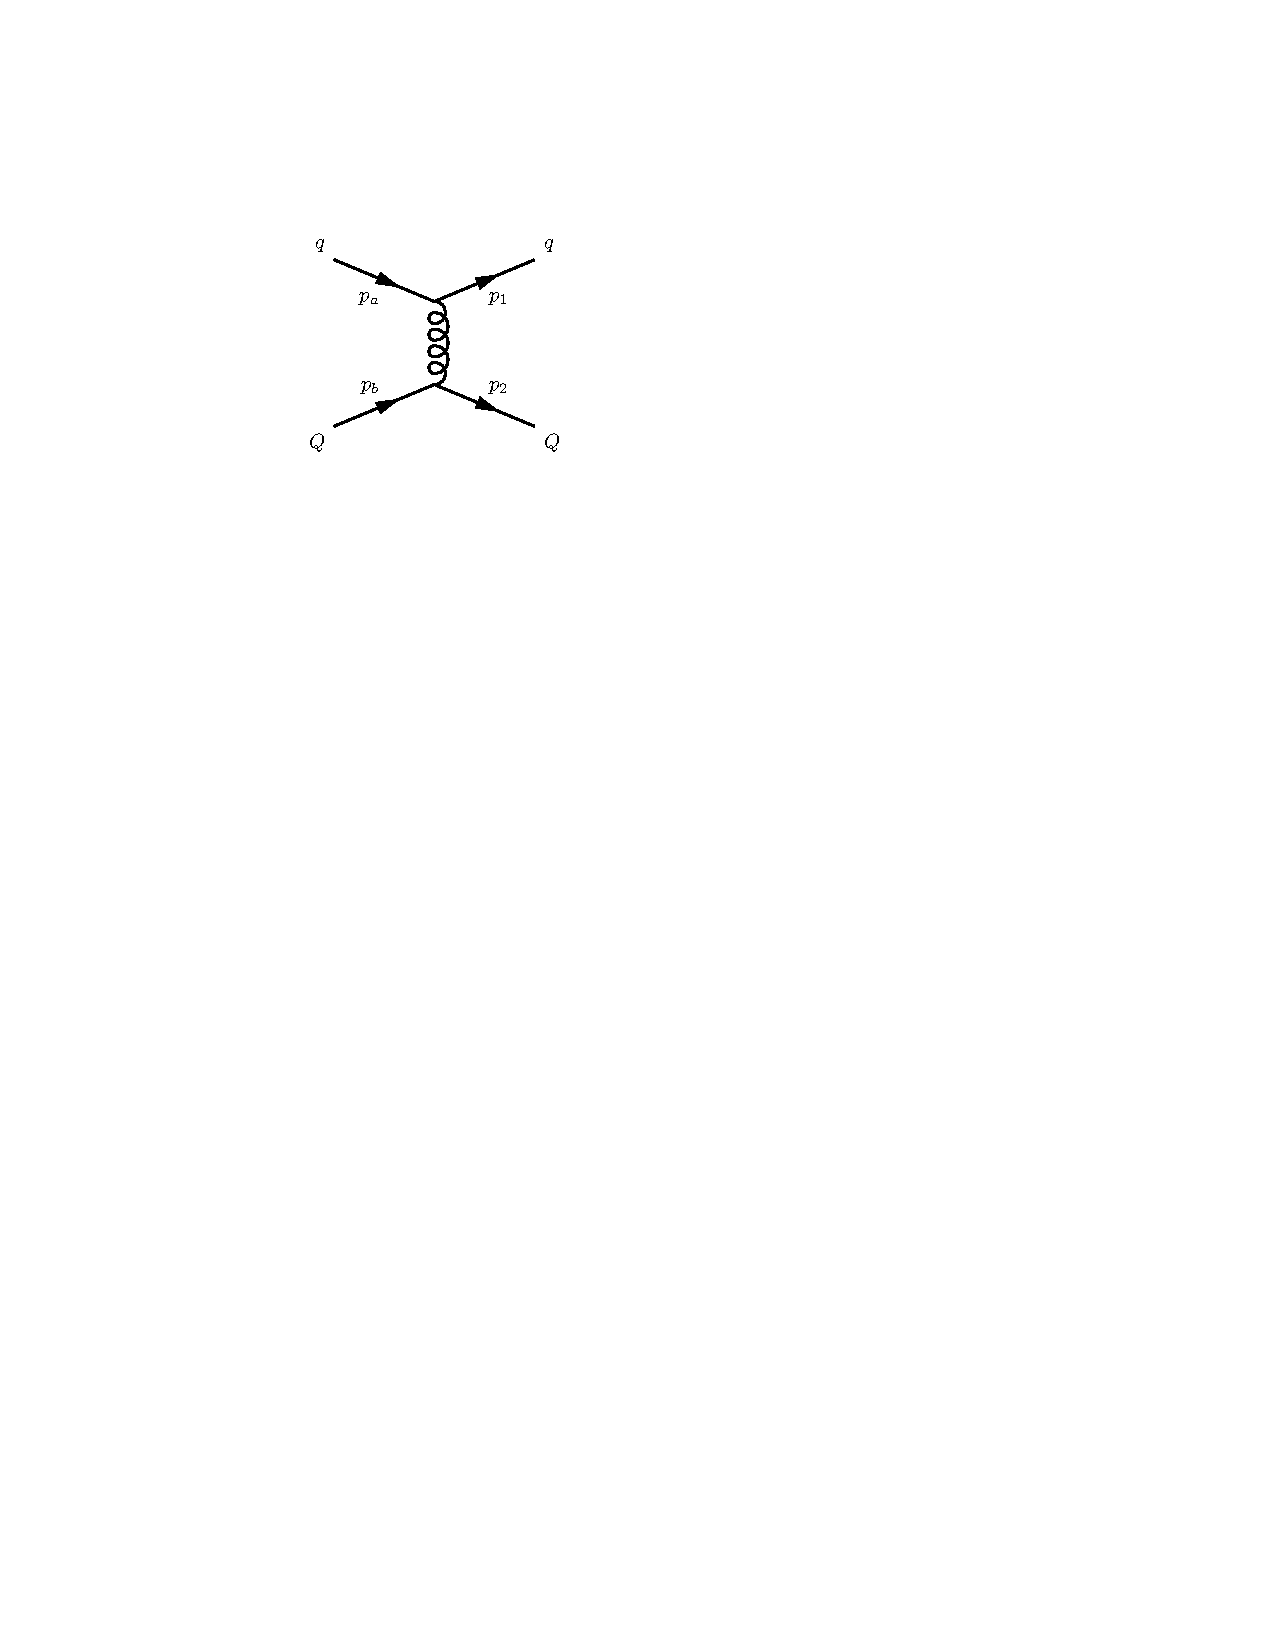
\includegraphics[width=0.35\linewidth]{TwoToTwo}
			\caption{The only diagram which contributes to $qQ\rightarrow qQ$ at leading order in $\alpha_s$.}
			\label{fig:TwoToTwo}
			\end{center}
		\end{figure}

	\section{$qg$ scattering at High Energy}

		We now explore the more involved case of $q^-g^+\to q^-g^+$ scattering.  At leading order this
		consists of three diagrams shown in fig.~\eqref{fig:TwoToTwo2}.  We use the following gauge
		choice for the gluon polarisations:

		\begin{align}
		\epsilon^{+*}_{2\sigma}&=\frac{\langle b|\sigma|2\rangle}{\sqrt{2}\langle b2\rangle}
		& \epsilon^{-*}_{2\sigma} &= -\frac{\langle b|\sigma|2\rangle}{\sqrt{2}[b2]} \\
		\epsilon^{+}_{b\sigma}&=-\frac{\langle b|\sigma|2\rangle}{\sqrt{2}[2b]}
		& \epsilon^{-*}_{2\sigma} &= -\frac{\langle b|\sigma|2\rangle}{\sqrt{2}\langle 2b\rangle}
		\end{align}

		For simplicity we choose to write everything in terms of negative helicity spinor-helicity brackets;
		to describe positive helicities we can use the transposition property of spinor-helicity brackets discussed
		in section~\ref{sec:SpinorHelicity}.

		\begin{figure}[h]
			\centering
			\begin{subfigure}[b]{0.3\textwidth}
				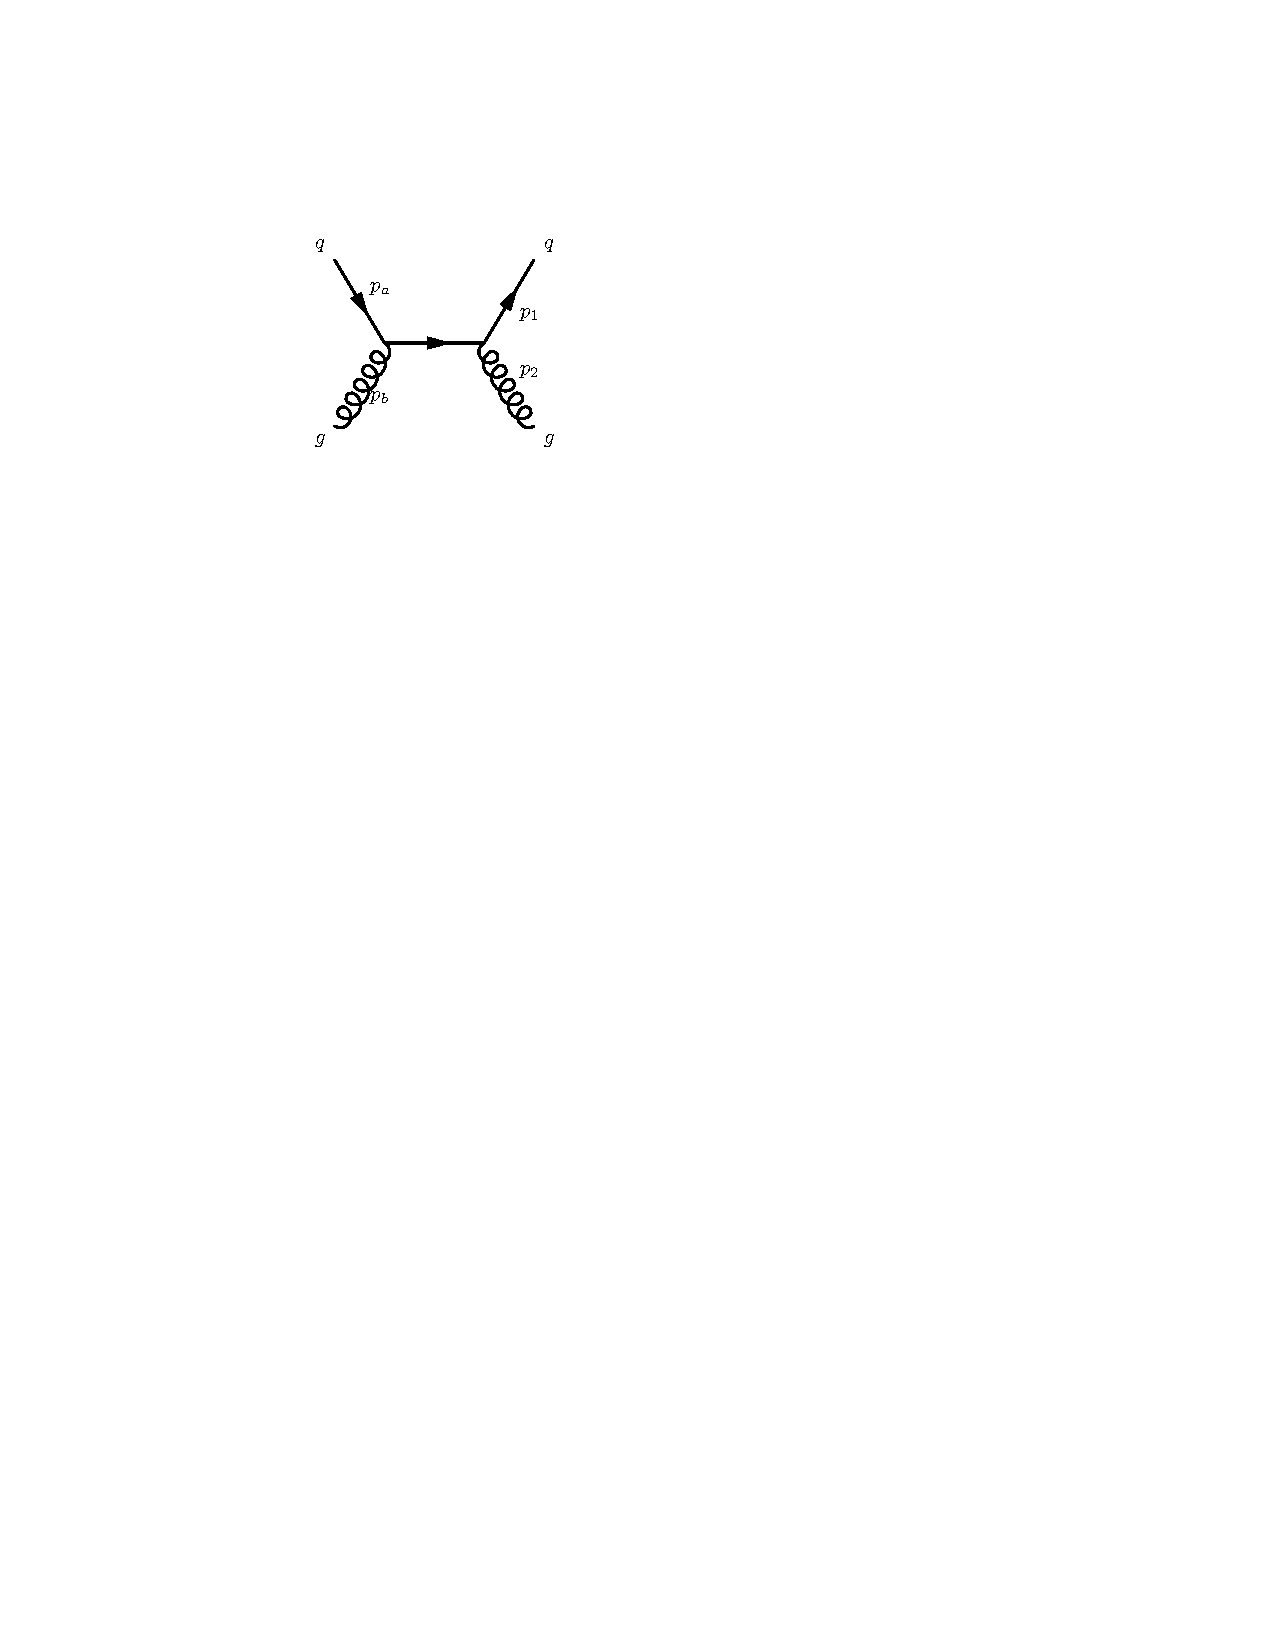
\includegraphics[width=\textwidth]{qg2qg-s}
				\caption{}
				\label{fig:qg2qg-s}
			\end{subfigure}

			\begin{subfigure}[b]{0.3\textwidth}
				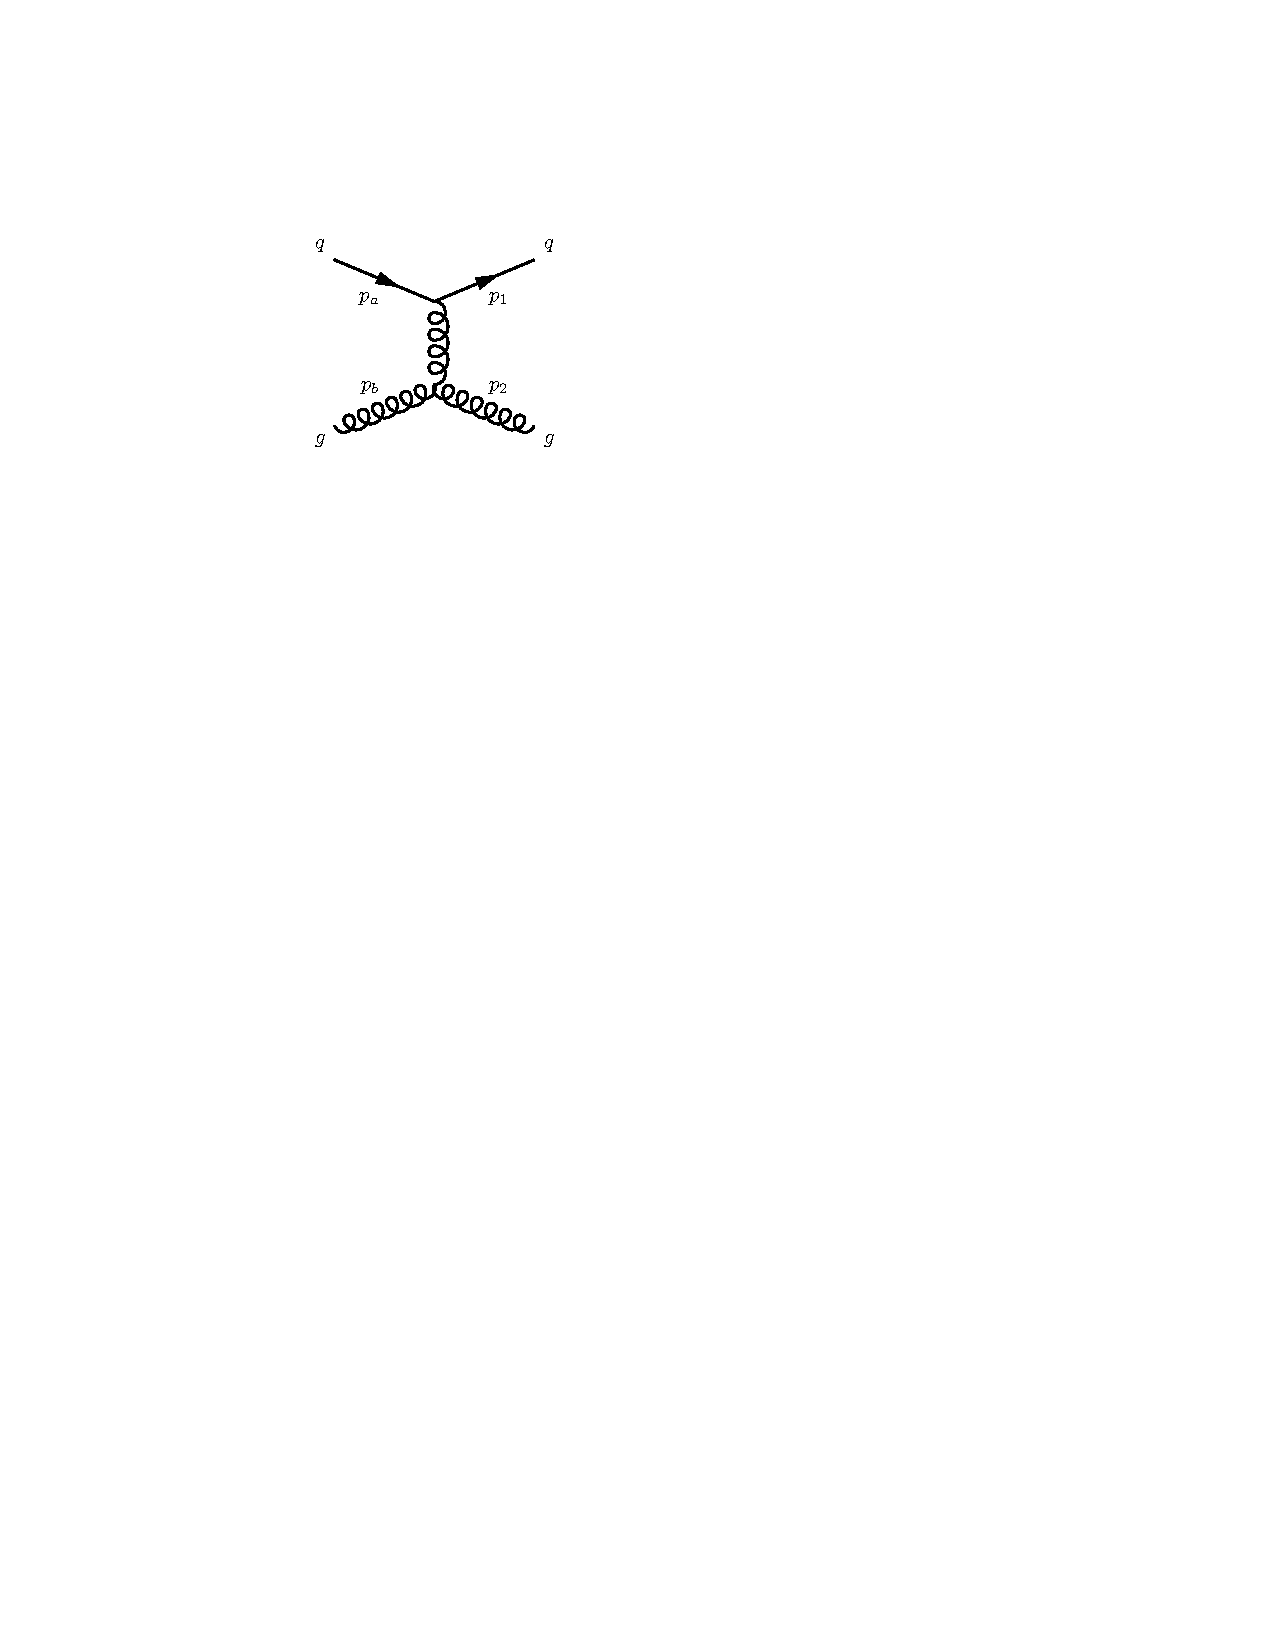
\includegraphics[width=\textwidth]{qg2qg-t}
				\caption{}
				\label{fig:qg2qg-t}
			\end{subfigure}
			~
			\begin{subfigure}[b]{0.3\textwidth}
				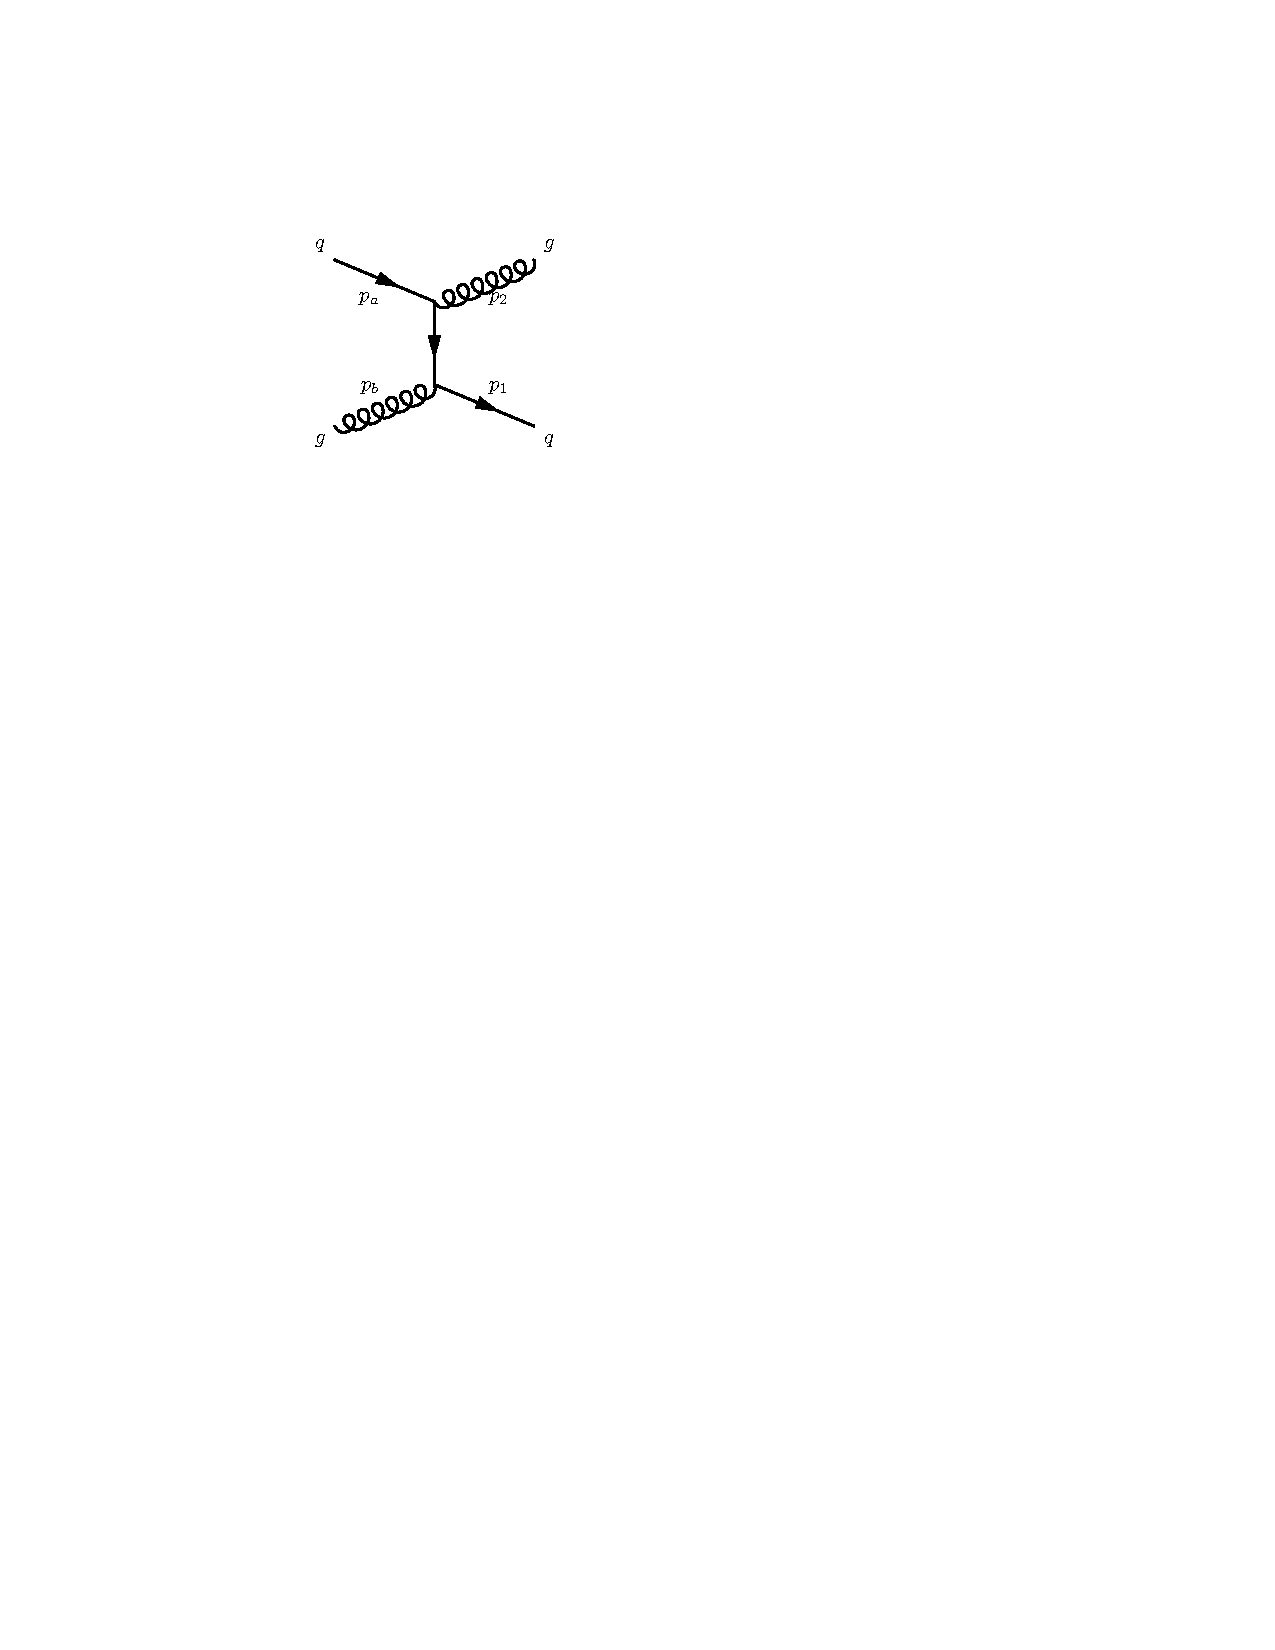
\includegraphics[width=\textwidth]{qg2qg-u}
				\caption{}
				\label{fig:qg2qg-u}
			\end{subfigure}
			\caption{The $s$, $t$ and $u$ channel diagrams contributing to $q^-g^+\to q^-g^+$ at leading
			         order in $\alpha_s$ in figures (\ref{fig:qg2qg-s}), (\ref{fig:qg2qg-t}) and (\ref{fig:qg2qg-u})
			         respectively.}
			\label{fig:TwoToTwo2}
		\end{figure}

		\subsection{$s$-channel}

			The matrix element for the $s$-diagram, shown in fig.~\eqref{fig:qg2qg-s}, is:

			\begin{align}
				\mathcal{M}_{q^-g^+\to q^-g^+, s}^{\text{LO}}=&T^b_{ae}T^2_{e1}\overline{u}^-(p_1)\left(-\frac{ig_s}{2}\gamma^\mu\right)\epsilon_\mu^{*+}(p_2)
					\frac{i(\slashed q+m)}{q^2-m^2}\left(-\frac{ig_s}{2}\gamma^\nu\right)\epsilon^+_\nu(p_b)u^-(p_a), \\
				=&-\frac{g^2_s}{4q^2}\epsilon^{*+}_{2\mu}\epsilon^+_{b\nu}\overline{u}^-_1\gamma^\mu\slashed q\gamma^\nu u^-_a,
			\end{align}

			where we have used $q\gg mc$ for the high energy case (i.e. we treat the quarks as massless in the High Energy limit).
			The propagator has momentum $q=p_a+p_b=p_1+p_2$ and therefore:

			\begin{align}
				\mathcal{M}_{q^-g^+\to q^-g^+, s}^{\text{LO}}=&-T^b_{ae}T^2_{e1}\frac{g^2_s}{4q^2}\frac{\langle{b}|\mu|2\rangle}{\sqrt{2}\langle{b2\rangle}}
				\frac{\langle{b}|\nu|2\rangle}{\sqrt{2}[2b]}\overline{u}^-_1\gamma^\mu(\slashed{p}_a+\slashed{p}_b)\gamma^\nu u^-_a.
			\end{align}

			Now we can use the completeness relations for $\slashed p_{a/b}$ and see that:

			\begin{equation}
				\mathcal{M}_{q^-g^+\to q^-g^+, s}^{\text{LO}}=-T^b_{ae}T^2_{e1}\frac{g^2_s}{4q^2t}[2a]\langle ab\rangle\langle{b}|\mu|2\rangle\langle{1}|\mu|a\rangle
			\end{equation}

			Using $q^2=s_{ab}=\langle ab\rangle[ba]$ and $t=\langle2b\rangle[b2]$ we have:

			\begin{equation}
			\mathcal{M}_{q^-g^+\to q^-g^+, s}^{\text{LO}}=-T^b_{ae}T^2_{e1}\frac{g^2_s}{4}\frac{[2a]\langle ab\rangle}{\langle ab\rangle[ba]
			\langle2b\rangle[b2]}\langle{b}|\mu|2\rangle\langle{1}|\mu|a\rangle.
			\end{equation}

			Now we must calculate the spinor products.  We use the conventions for spinors outlined in the
			previous chapter.  For example:

			\begin{align}
				[2a] = &\overline{u}^+_2u^-_a=-\frac{\sqrt{p_a^+p_2^-}p_2^\perp}{|p_2^\perp|},
			\end{align}

			and after calculating the other brackets we see:

			\begin{equation}
				\mathcal{M}_{q^-g^+\to q^-g^+, s}^{\text{LO}} = -T^b_{ae}T^2_{e1}\frac{g_s^2}{4}\sqrt{\frac{p_2^-}{p_b^-}}\frac{1}{p_2^+p_b^-} \frac{p_{2\perp}^*}{|p_{2\perp}|} \bk{b}{\mu}{2} \bk{1}{\mu}{a}
			\end{equation}

			Which can be simplified to give the final result:

			\begin{equation}
				\mathcal{M}_{q^-g^+\to q^-g^+, s}^{\text{LO}}=-T^b_{ae}T^2_{e1}\frac{g_s^2}{2\hat{t}}\sqrt{\frac{p_2^-}{p_b^-}}\frac{p_{2\perp}^*}
				{|p_{2\perp}|}\langle{b}|\mu|2\rangle\langle{1}|\mu|a\rangle
				\label{eqn:s-channel}
			\end{equation}

		\subsection{$t$-channel}

			The matrix element for the $t$-channel diagram, shown in fig.~\eqref{fig:qg2qg-t}, is:

			\begin{align}
			\begin{split}
				-i\mathcal{M}_{q^-g^+\to q^-g^+, t}^{\text{LO}} =
				&-T^e_{a1}f^{b2e}\overline{u}^-_1\Bigg(-\frac{ig_s}{2}\gamma^\mu\Bigg)\Bigg(-\frac{ig_{\mu\nu}}{q^2}\Bigg)u^-_ag_s\\
				&\Big(g_{\sigma\nu}(p_b-q)_\rho + g_{\nu\rho}(q+p_b)_\sigma - g_{\rho\sigma}(p_b+p_2)_\nu)\Big)\epsilon^{\rho *}_{2+}\epsilon^{\sigma}_{b+}\\
			\end{split}
			\end{align}

			Now using $q=p_2-p_b$ and $p_2\cdot\epsilon_2 = p_b\cdot\epsilon_b = 0$:

			\begin{align}
			\begin{split}
				-i\mathcal{M}_{q^-g^+\to q^-g^+, t}^{\text{LO}} =
			        -T^e_{a1}f^{b2e}\frac{g_s^2}{2q^2s_{2b}}\left(\overline{u}^-_1\gamma^{\nu}u^-_a\right)\left(\overline{u}^-_b\gamma^{\rho}u^-_2\right)\left(\overline{u}^-_b\gamma^{\sigma}u^-_2\right)\\
				\Big(2g_{\sigma\nu}p_{b\rho} + 2g_{\nu\rho}p_{2\sigma} - g_{\rho\sigma}(p_b+p_2)_\nu\Big),
			\end{split}
			\end{align}

			which cancels completely and therefore:

			\begin{equation}
				\mathcal{M}_{q^-g^+\to q^-g^+, t}^{\text{LO}}=0,
				\label{eqn:t-channel}
			\end{equation}

			in this gauge.

		\subsection{$u$-channel}

			The matrix element for the $u$-diagram, shown in fig.~\eqref{fig:qg2qg-t}, is:

			\begin{equation}
				\begin{split}
				-i\mathcal{M}_{q^-g^+\to q^-g^+, u}^{\text{LO}} &= T^2_{ae}T^b_{e1}\overline{u}^-(p_1)\left(-\frac{ig_s}{2}\gamma^\mu\right)
				\frac{i(\slashed q+mc)}{q^2-m^2c^2}\left(-\frac{ig_s}{2}\gamma^\nu\right)u^-(p_a)\epsilon_\mu^{*+}(p_b)\epsilon^+_\nu(p_2)\\
				\mathcal{A}_u &= \frac{g_s^2}{4q^2}\overline{u}^-_1\gamma^\mu\slashed q\gamma^\nu u^-_a\epsilon^{+*}_{b\mu}\epsilon^*_{2\nu}\\
				&= \frac{g_s^2}{8q^2s_{2b}}\langle b|\mu|2\rangle\langle b|\nu|1\rangle\overline{u}^-_1\gamma^\mu(\slashed{p}_a-\slashed{p}_2)\gamma^\nu u^-_a\\
				\end{split}
			\end{equation}

			Where we have used $q=p_a-p_2$.  By direct comparison with the procedure used for the $s$-channel we can see the result will be:

			\begin{equation}
			\mathcal{M}_{q^-g^+\to q^-g^+, u}^{\text{LO}}=
			T^2_{ae}T^b_{e1}\frac{g_s^2}{2\hat{t}}\sqrt{\frac{p_b^-}{p_2^-}}\frac{p^*_{2\perp}}{|p_{2\perp}|}\langle{b}|\mu|2\rangle\langle{1}|\mu|a\rangle.
			\label{eqn:u-channel}
			\end{equation}

			The total total matrix element is given by the sum of eqs.~\eqref{eqn:s-channel},~\eqref{eqn:t-channel} and~\eqref{eqn:u-channel} which is:

			\begin{equation}
				\mathcal{M}_{q^-g^+\to q^-g^+}^{\text{LO}}
				\frac{g_s^2}{2}\frac{p_{2\perp}^*}{|p_{2\perp}|}\left(T^2_{ae}T^b_{e1}\sqrt{\frac{p_b^-}{p_2^-}}-T^b_{ae}T^2_{e1}
				\sqrt{\frac{p_2^-}{p_b^-}}\right)\frac{\langle{b}|\mu|2\rangle\langle{1}|\mu|a\rangle}{\hat{t}},
				\label{eqn:fullsum}
			\end{equation}

			We also see that eqn.~\eqref{eqn:fullsum} has the same spinor-helicity brackets contracted as eqn.~\eqref{eqn:similarBrackets}
			and so the dominant behaviour of $q^-g^+\to q^-g^+$ in the high energy limit is $\frac{s}{t}$.
			In the High Energy limit we have $p_b^-\thicksim p_2^-$ and so eqn.~\eqref{eqn:fullsum} could be simplified
			further to:

			\begin{equation}
				\mathcal{M}_{q^-g^+\to q^-g^+}^{\text{LO}}=i\frac{g_s^2}{2}\frac{p_{2\perp}^*}{|p_{2\perp}|}f^{2bc}T^c_{a1}
				\frac{\langle{b}|\mu|2\rangle\langle{1}|\mu|a\rangle}{\hat{t}}.
				\label{eqn:fullsum2}
			\end{equation}

			which is identical to the result found in the previous $qQ\rightarrow qQ$ calculation (save for a phase which cancels
			at the amplitude squared level). Since the kinematics of which is exactly in the form of two `currents' contracted as
			seen in section~\ref{sec:qQScat}.  We have:

			\begin{equation}
				\mathcal{M}_{qg\to qg}^{\text{LO}} = \frac{C_A}{C_f} \mathcal{M}_{qQ\to qQ}^{\text{LO}},
			\end{equation}

			in the High Energy limit. In practice we actually choose \emph{not} to take the High Energy limit to obtain
			eqn.~\eqref{eqn:fullsum2} so as to approximate as little as possible.  Even without this extra approximation
			eqn.~\eqref{eqn:fullsum} is still exactly the form of a $t$-channel gluon exchange we saw in
			eqn.~\eqref{eqn:similarBrackets}.

	\section{Factorisation Into Currents}
		\label{sec:currents}

		While one could argue that the fact that the $qQ\to qQ$ matrix element would factorise into a
		contraction of two vector currents with a $t$-channel pole was obvious (since the only
		contribution was from a $t$-channel diagram!), it was not at all obvious that this
		would also be the case for the $qg\to qg$ amplitude would.  It can also be shown that
		the same structure is found even in the case of gluon-gluon scattering\cite{Andersen:2011hs}.

		It turns out that this factorisation into a form with only a $t$-channel pole holds for
		all the helicity configurations where the helicities of the incoming-outgoing parton lines
		remain unchanged.  For those diagrams where the helicity \emph{is} flipped we find poles
		in $s$ and $u$ and so these contributions are heavily suppressed in the High Energy limit.
		The fact that all of the approximate helicity averaged matrix elements squared for any combination
		of incoming partons, $a$ and $b$, can be written as:

		\begin{equation}
			|\bar{\mathcal{M}}_{2\to2}| \sim \sum_{h_a, h_b, h_1, h_2}
			\left|\frac{j^\mu_a(p_a, p_1)\ j_{b, \mu}(p_b, p_2)}{t}\right|^2,
		\end{equation}

		is exploited in \hej to express more general matrix elements (those with higher multiplicity or
		more complicated final states) approximately.

		By constructing a current describing, for example, a $W^\pm$ boson being emitted from an
		incoming-outgoing quark line we can then write down the matrix element for the process
		$q'q\to(W^\pm\to)\nu e^\pm q'Q$ as:

		\begin{equation}
			|\bar{\mathcal{M}}_{2\to2}|^2 \sim \sum_{h_a, h_b, h_1, h_2, h_{e^\pm}, h_\nu}
			\left|\frac{j^\mu_{W^\pm}(p_a, p_1, p_{e^\pm}, p_\nu)\ j_\mu(p_b, p_2)}{t}\right|^2,
			\label{eqn:wExample}
		\end{equation}

		where the quark line which emitted the $W^\pm$ has changed flavour from $q$ to $Q$.  Eqn.~\eqref{eqn:wExample}
		is an approximation which, technically, is only valid in the strict limit of infinite invariance mass between
		the outgoing quarks however, as we will see later, this approximation does a remarkably good job at
		describing data far away from its formal region of applicability.

		% It should not come as a surprise that the $qQ\rightarrow qQ$ and $qg\rightarrow qg$ channels closely resemble
		% each another since if we consider the sub-diagrams involved in the $t$-channel exchange namely the quark and
		% gluon `currents' in the high energy limit we see that they themselves are similar.  The gluon emission
		% current, $j_{g}^\sigma$, shown in fig. (Is this a figure worth having?) is given by

		% \begin{equation}
		% 	j_{g}^\sigma = \left((p_a+p_1)^\sigma g^{\mu\nu} + (q - p_1)^\mu g^{\nu\sigma} -
		% 	(q + p_a)^\nu g^{\mu\sigma}\right)\epsilon_{a, \mu}\epsilon_{1, \nu}^*.
		% \end{equation}

		% In the High Energy limit we can take $p_a\sim p_1$ and therefore this becomes:

		% \begin{equation}
		% 	j_{g}^\sigma \sim \left(2p_a^\sigma g^{\mu\nu} - p_a^\mu g^{\nu\sigma} -
		% 	p_1^\nu g^{\mu\sigma}\right)\epsilon_{a, \mu}\epsilon_{1, \nu}^*.
		% \end{equation}

		% But the second and third terms here are zero once we take the contraction with the gluon polarisations
		% $\epsilon_{a, \mu}$ and $\epsilon_{1, \nu}^*$ respectively so we are left with simply:

		% \begin{equation}
		% 	j_{g}^\sigma \sim 2p_a^\sigma\epsilon_{a}^\mu\cdot\epsilon_{1, \mu}^*.
		% 	\label{eqn:gluonCurrent}
		% \end{equation}

		% If we compare this to the quark current, $j_{q}^\sigma$, shown in fig. (Is this a figure worth having?),
		% which is given by:

		% \begin{equation}
		% 	j_{q}^\sigma = \bk{1}{\sigma}{a},
		% \end{equation}

		% and using the spinor-helicity property for spinors with the same momenta:

		% \begin{equation}
		% 	j_{q}^\sigma \sim 2p_a^\sigma
		% \end{equation}

		% which is identical to~\eqref{eqn:gluonCurrent} aside from a scalar gauge-dependent term.

		In what follows we construct high multiplicity matrix elements by approximating the full result
		by the contraction of two currents and a number of effective vertices.  This choice allows us
		to construct matrix elements with a simple form which contains the leading logarithms by
		ensuring that they have the maximal number of gluons exchanged in the $t$-channel.\\
		As a simple example we consider the production of 4 exclusive jets in the High Energy limit.
		Fig.~\eqref{fig:quadJets} shows three diagrams which all contribute at leading order in $\alpha_s$;
		fig.~\eqref{fig:quadJets1} has three gluons exchanged in the $t$-channel and so its amplitude will
		have propagator terms akin to:

		\begin{equation}
			\mathcal{M}_{\text{(a)}}\sim\frac{1}{(p_a - p_1)^2(p_a - p_1 - p_2)^2(p_a - p_1 - p_2 - p_3)^2},
			\label{eqn:inPlace}
		\end{equation}

		arising from the gluon propagators.  By contrast figs.~\eqref{fig:quadJets2} and~\eqref{fig:quadJets3} will
		have, in place of~\eqref{eqn:inPlace}:

		\begin{align}
			\mathcal{M}_{\text{(b)}}\sim\frac{\slashed p_a - \slashed p_1}
			{(p_a - p_1)^2(p_a - p_1 - p_2)^2(p_a - p_1 - p_2 - p_3)^2},\\
			\intertext{and,}
			\mathcal{M}_{\text{(c)}}\sim\frac{(\slashed p_a - \slashed p_1)(\slashed p_4 - \slashed p_b)}
			{(p_a - p_1)^2(p_a - p_1 - p_2)^2(p_a - p_1 - p_2 - p_3)^2},
		\end{align}

		\begin{figure}[bt]

			\centering

			\begin{subfigure}[b]{0.31\textwidth}
				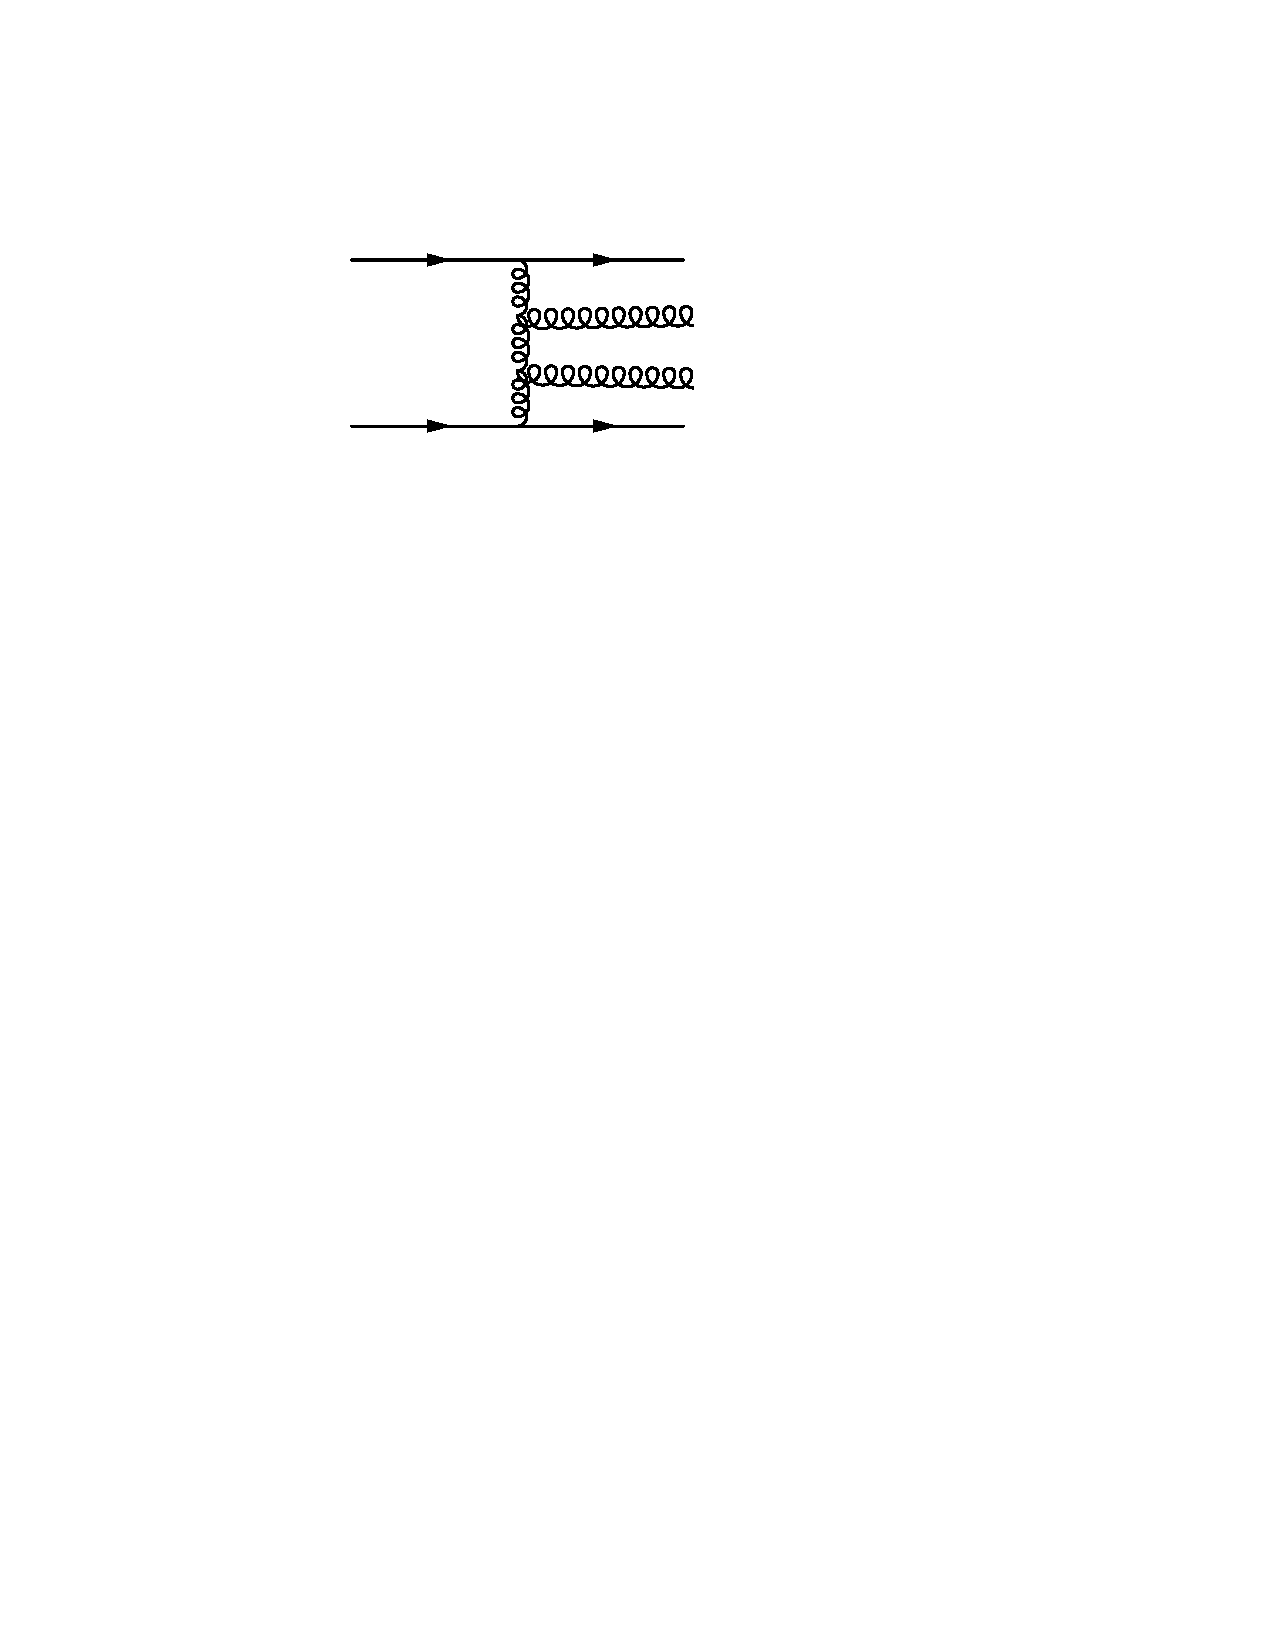
\includegraphics[width=\textwidth]{quadJets1}
				\caption{}
				\label{fig:quadJets1}
			\end{subfigure}
			\begin{subfigure}[b]{0.31\textwidth}
				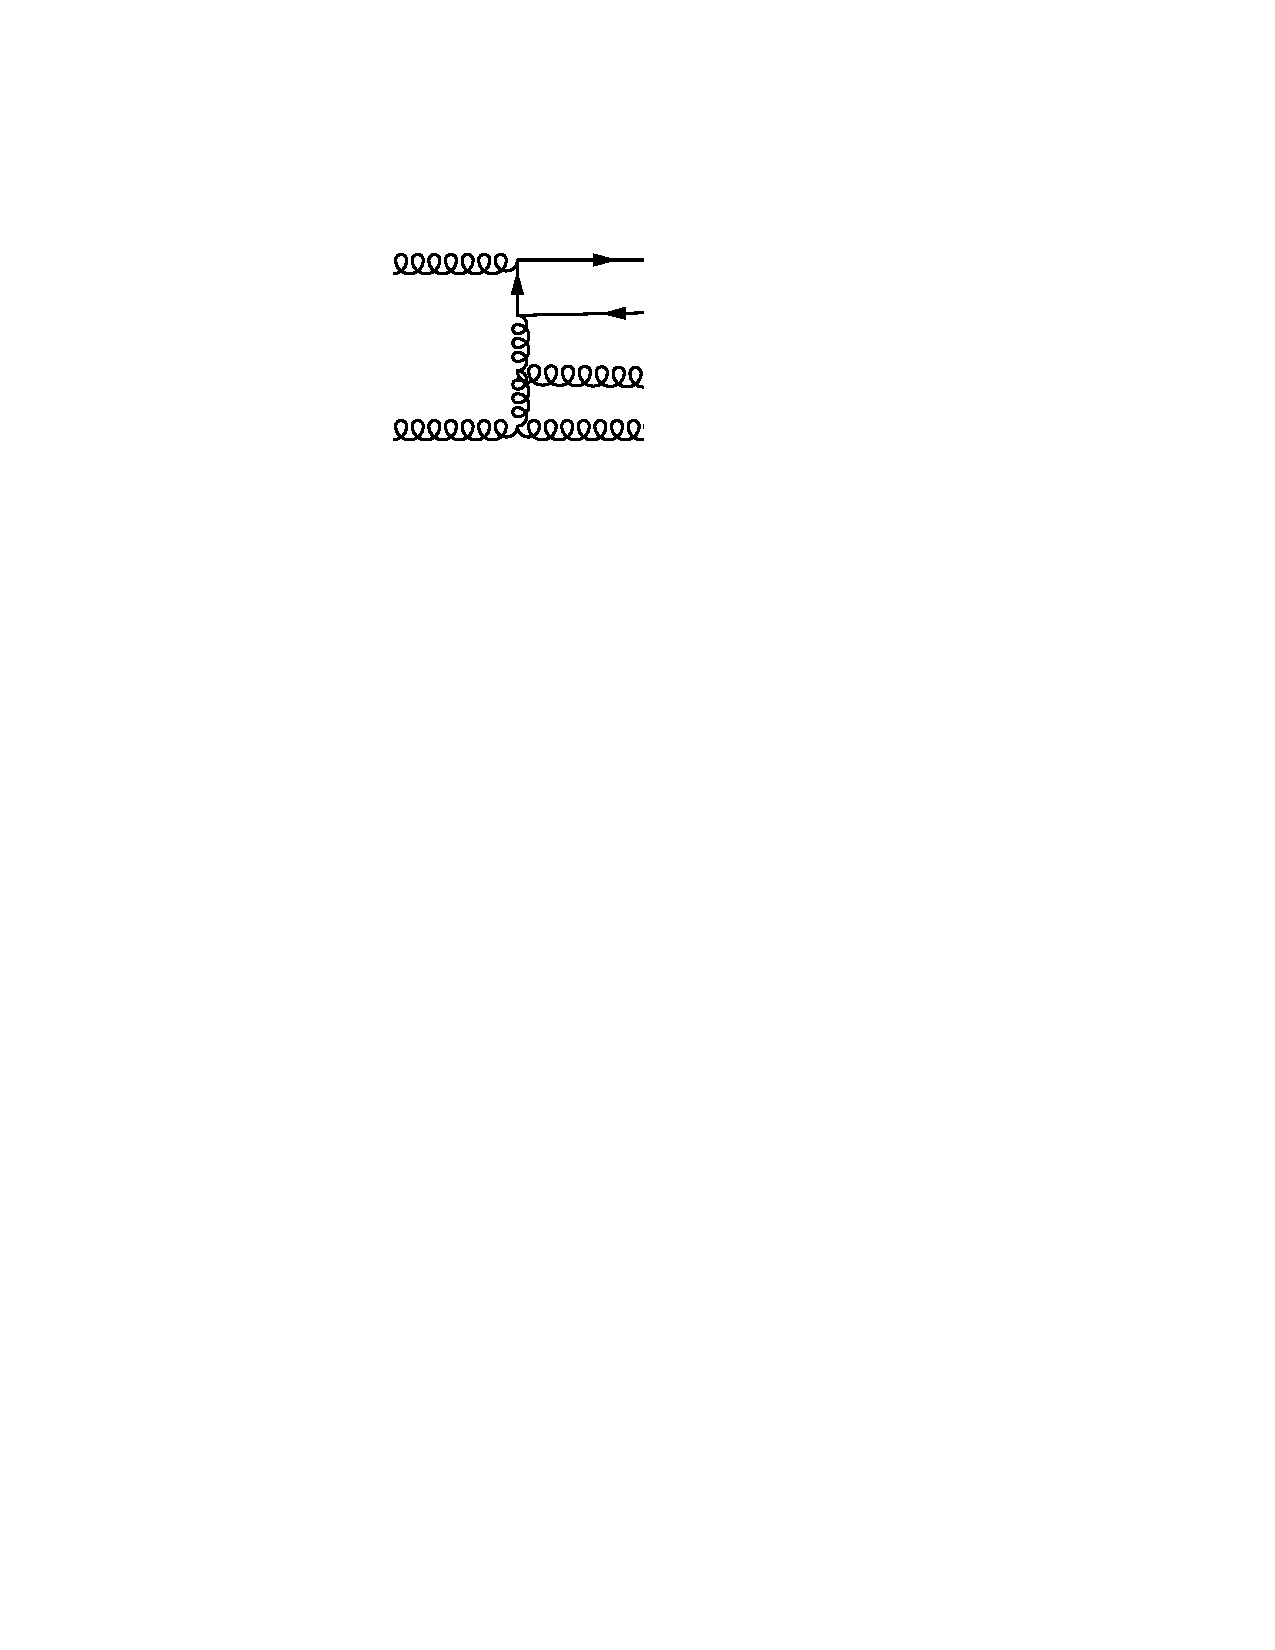
\includegraphics[width=\textwidth]{quadJets2}
				\caption{}
				\label{fig:quadJets2}
			\end{subfigure}
			\begin{subfigure}[b]{0.31\textwidth}
				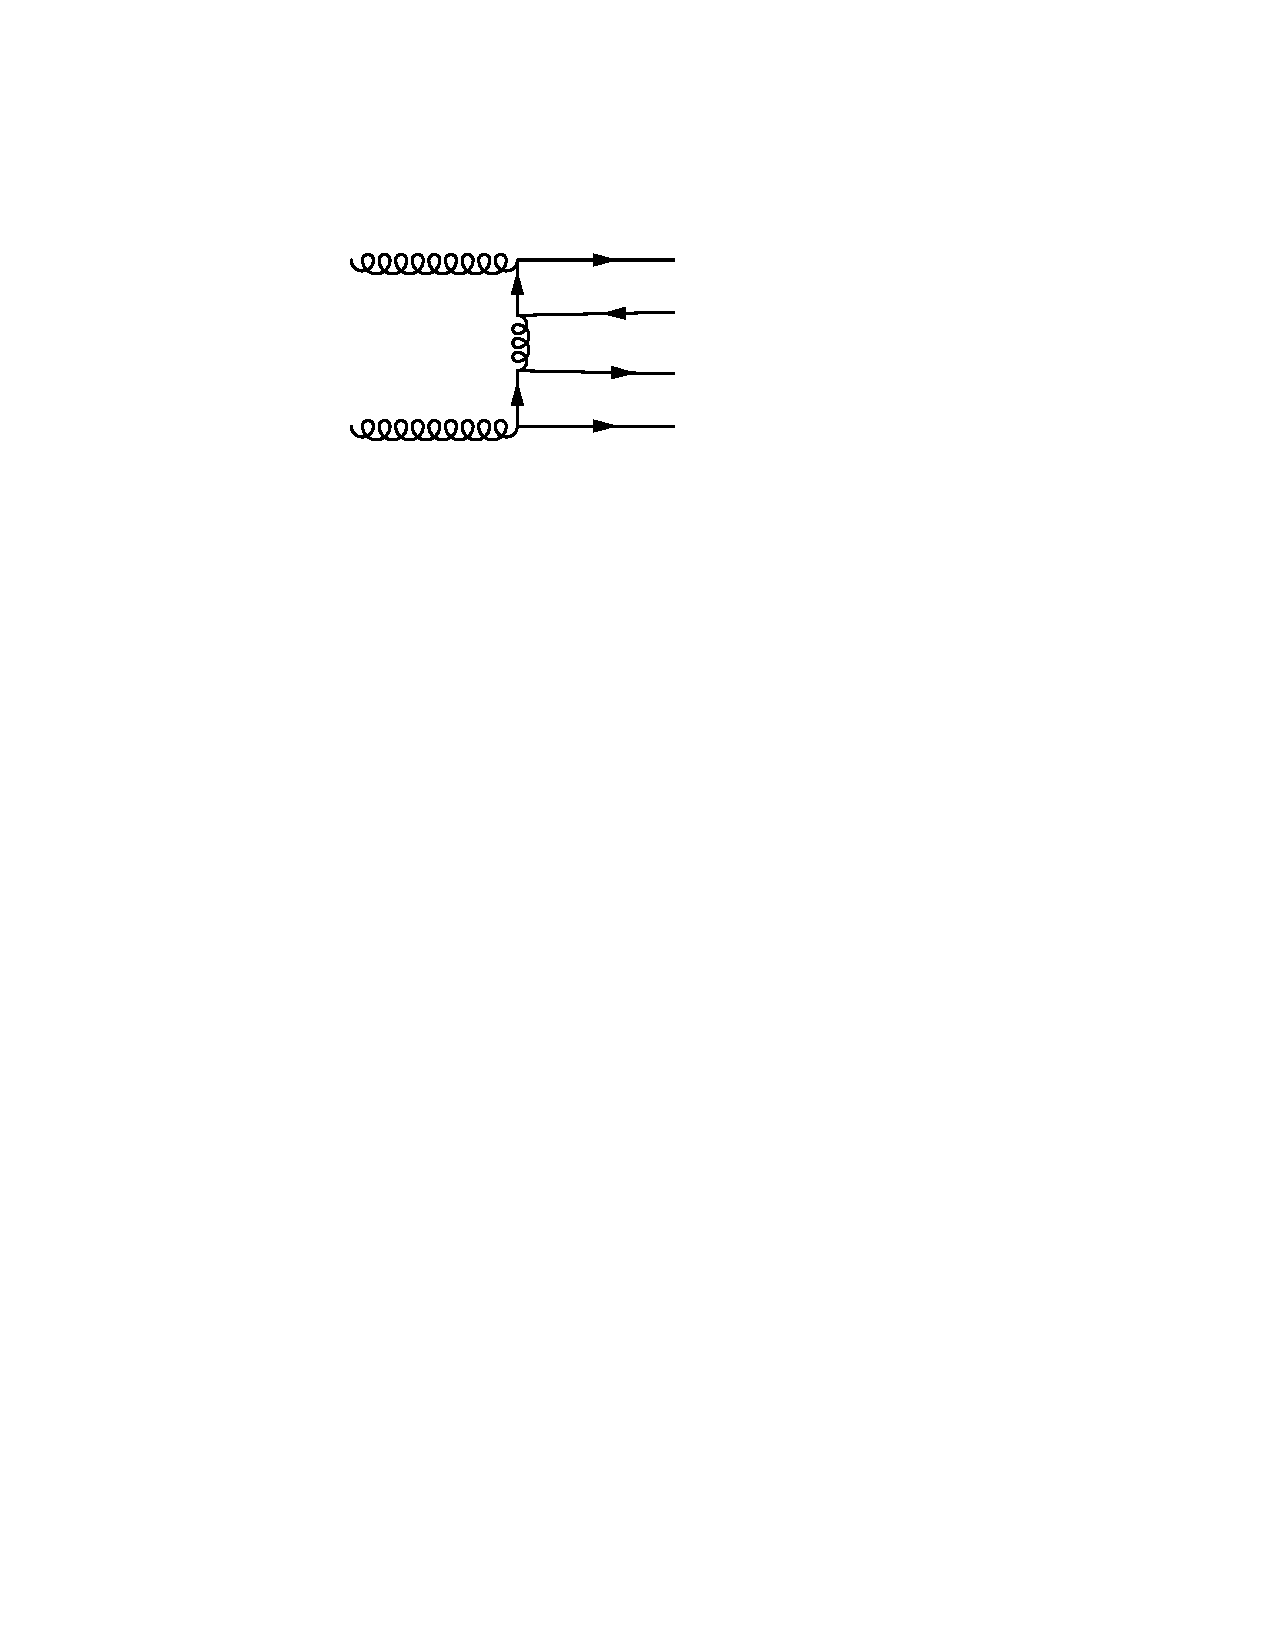
\includegraphics[width=\textwidth]{quadJets3}
				\caption{}
				\label{fig:quadJets3}
			\end{subfigure}

			\caption{Three processes contributing to exclusive quad-jet production. (a) has the
			maximum number of gluons exchanged in the $t$-channel (three) and will dominate in the High
			Energy limit, (b) and (c) only have two and one gluon which can reggeise.  As such as we move
			from left to right we will lose powers of large logarithms but maintain the same power of
			$\alpha_s$ and therefore we can reasonably approximate quad-jet production by neglecting
			(b) and (c).}
			\label{fig:quadJets}
		\end{figure}

		respectively.  Since in the High
		Energy limit we have $p_a\sim p_1$ and $p_b\sim p_4$ it is clear that $\mathcal{M}_{\text{(b)}}$
		and $\mathcal{M}_{\text{(c)}}$ will be suppressed with respect to $\mathcal{M}_{\text{(a)}}$.
		Clearly this only a heuristic argument but it is sufficient to motivate the construction of
		high multiplicity amplitudes from $t$-channel gluon exchanges with the understanding that any
		other diagrams will be formally sub-leading.  We call the configurations with a maximal
		number of gluons exchanged in the $t$-channel an `FKL' configuration;  For example
		fig.~\eqref{fig:quadJets1} is an FKL configuration while fig.~\eqref{fig:quadJets2} and fig.
		\eqref{fig:quadJets3} are `non-FKL' configurations.

		A more formal argument for which processes dominate in this limit was given by Fadin and Lipatov
		\cite{Kuraev:1976ge,Balitsky:1978ic}.  They found that, in the High Energy limit, scattering
		amplitudes scaled in the same way as was predicted by Regge theory.  This states that in the
		large invariant mass region a $2\to n$ matrix element has a limiting behaviour determined by
		the maximum spin of any particle which could be exchanged in the $t$-channel between final
		state partons neighbouring in rapidity.  We can then find the scaling of a process, for example
		$qg\to qg$, in particular regions of phase space where either $y_g\gg y_q$ or $y_q\gg y_g$ simply
		by drawing the associated colour connection diagrams for it.  This is shown in~\eqref{fig:colorConns}.
		Since when we have $y_g\gg y_q$ it is only possible to exchange a colour triplet (with spin one half)
		the cross-section will be dominated by the region where $y_q\gg y_g$.  The case for $2\to n$ is similar
		with the limiting behaviour of the matrix element given by

		\begin{equation}
			\mathcal{M}^{\text{HE}}_{2\to n}\sim s_{12}^{\omega_1}\cdots s_{(n-1)n}^{\omega_{(n-1)}}.
			\label{eqn:reggeScaling}
		\end{equation}

		Eqn.~\eqref{eqn:reggeScaling} now makes the previous discussion regarding figs.~\eqref{fig:quadJets}
		formally clear since fig.~\eqref{fig:quadJets1} will scale like:

		\begin{equation}
			\mathcal{M}^{\text{HE}}_{2\to 4} \sim s_{12}s_{23}s_{34},
		\end{equation}

		in the High Energy limit while figs.~\eqref{fig:quadJets2} and~\eqref{fig:quadJets3} will scale
		like:

		\begin{align}
		\begin{split}
			\mathcal{M}^{\text{HE}}_{2\to 4} \sim s_{12}^{\nicefrac{1}{2}}s_{23}s_{34},\\
			\mathcal{M}^{\text{HE}}_{2\to 4} \sim s_{12}^{\nicefrac{1}{2}}s_{23}s_{34}^{\nicefrac{1}{2}},
		\end{split}
		\end{align}

		respectively.  Since $s_{ij}$ are all large here, the processes with a (anti)quark exchanged
		in the $t$-channel will be high suppressed.

		\begin{figure}
			\begin{center}
			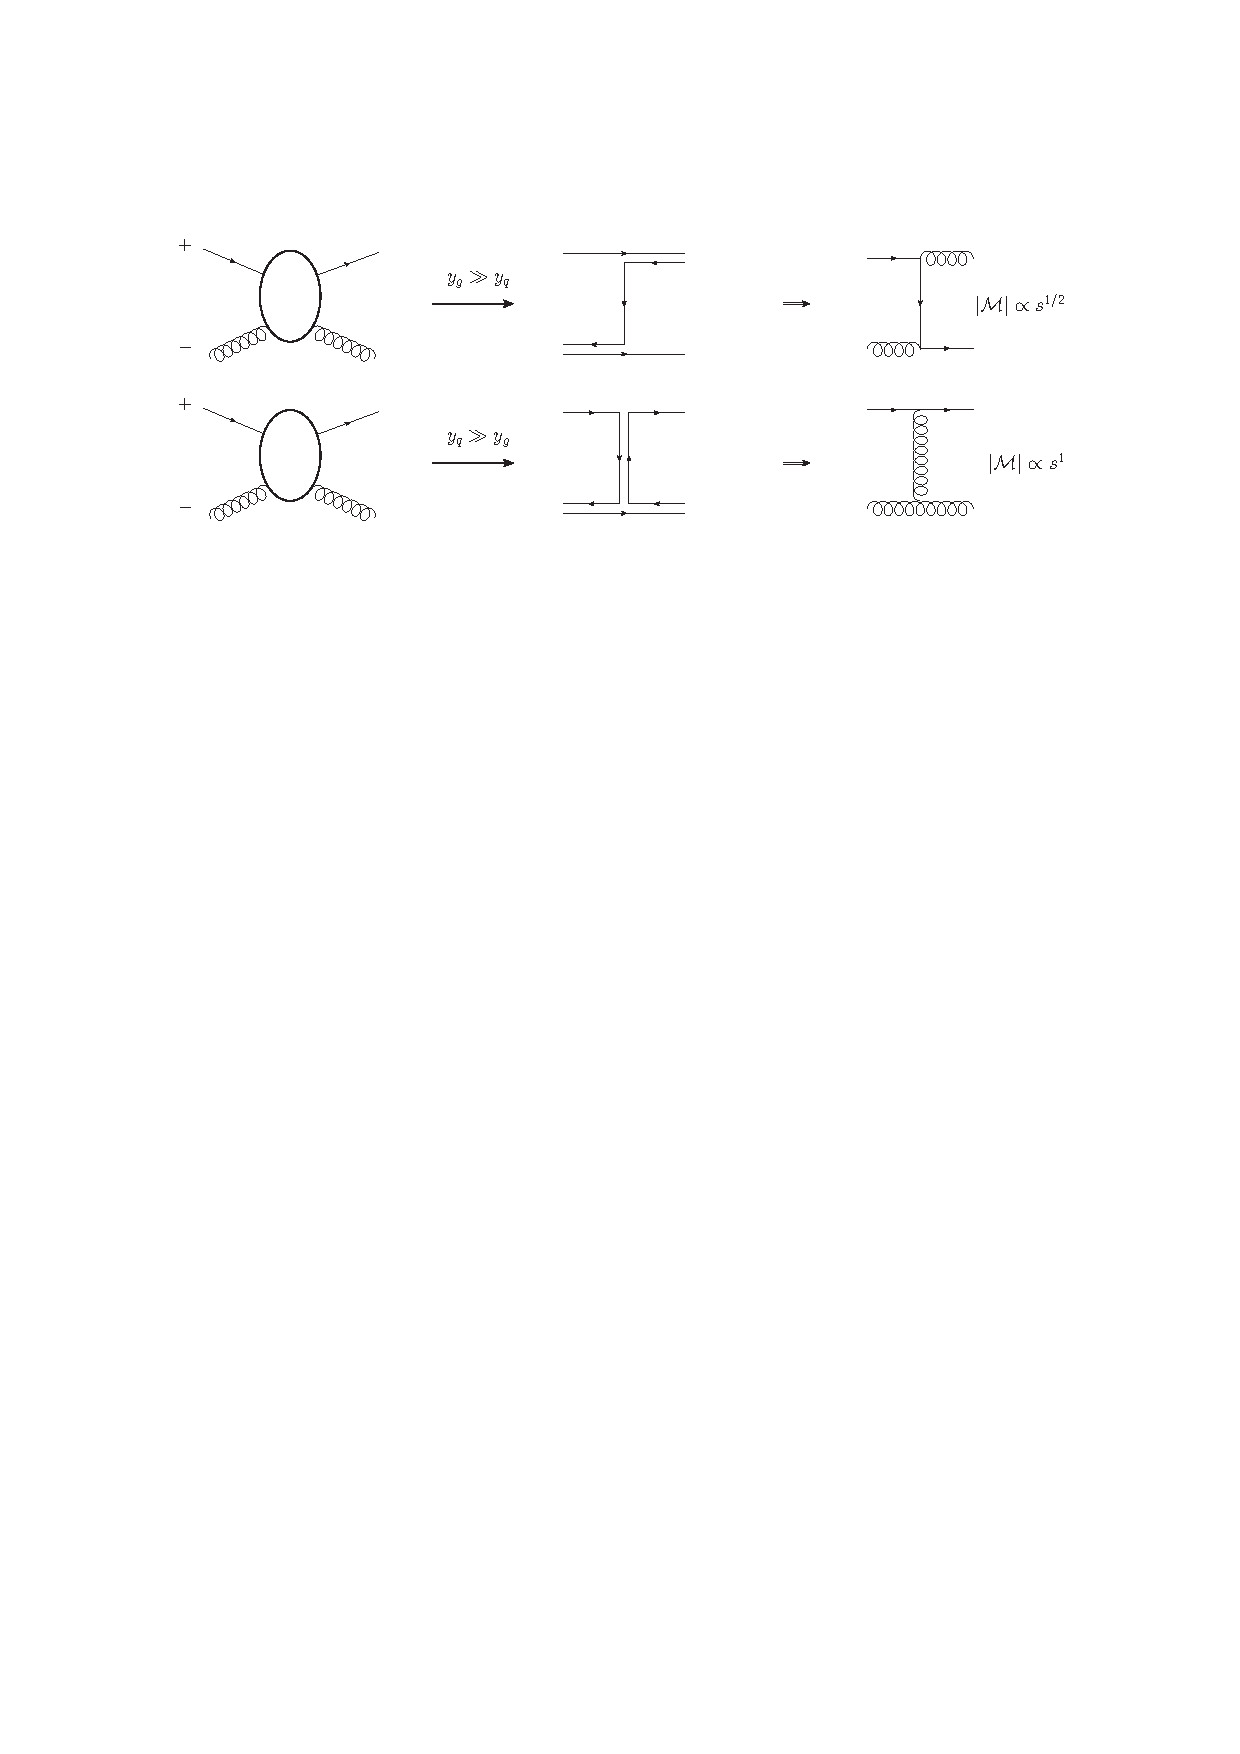
\includegraphics[width=1.0\linewidth]{ColourConns}
			\caption{The limiting behaviour of $qg\to qg$ in the regions of phase space where
			either $y_g\gg y_q$ or $y_q\gg y_g$.  The intermediate diagrams indicate the flow
			of colour through the process.}
			\label{fig:colorConns}
			\end{center}
		\end{figure}

		Here is a convenient place to define the `$t$-channel factorised' form for matrix elements,
		$\overline{\mathcal{M}}^t_{qQ\rightarrow qQ}$, in which we extract the $t$ poles from the
		rest of the matrix element \cite{Andersen:2009nu}.  We write the square of
		eqn.~\eqref{eqn:similarBrackets} as:

		\begin{equation}
			|\overline{\mathcal{M}}^t_{qQ\rightarrow qQ}|^2 = \frac{1}{4(N_c^2-1)}
			\frac{g^2C_F}{t_1}\frac{g^2C_F}{t_2} \sum_{h_a, h_b, h_1, h_2}
			|S_{qQ\rightarrow qQ}^{h_ah_b\rightarrow h_1h_2}|^2,
			\label{eqn:factorised}
		\end{equation}

		where $N_c=3$ and $C_F=\nicefrac{4}{3}$ for QCD, $S$ is the matrix element for a $2\rightarrow2$ process
		in the form of a contraction of two currents, and $t_i$ are the squared $t$-channel momenta - in this
		case $t_1=(p_a-p_1)^2$ and $t_1=(p_2-p_b)^2$.  While for this example eqn.~\eqref{eqn:factorised} is
		just an exact rewriting of a previous result we will use the form shown here to generalise to describing
		extra final state radiation in the next section at which point the $t$-channel factorisation weakens to
		an approximation of the full result (but one which contains enough of the underlying physics to be useful
		nonetheless).

	\section{$qQ$-scattering at High Energy (at NLO)}
		\label{sub:HE22_NLO}

		Before we continue on to look at how we might construct high multiplicity scattering matrix
		elements in terms of `currents' and effective vertices we briefly look at higher order (in
		$\alpha_s$) corrections to the process we studied in section~\ref{sec:qQScat}.
		So far we have seen the leading order \emph{processes} with a $t$-channel exchange are enhanced (as a result
		of Regge theory) but in
		eqn.~\eqref{eqn:schematicExpn} we sketched out a form for the perturbative expansion which also
		had enhanced higher order (in $\alpha_s$) terms.  We might na\"ively expect that the next-to-leading
		order diagrams with the most $t$-channel exchanges will give the greatest enhancement and, indeed,
		this turns out to be the case.  These diagrams are shown for the case of $qQ\rightarrow qQ$ in fig.
		\eqref{fig:NLO-leadingContrib}. The full calculation can be found in \cite{DelDuca:1995hf} (for
		the case of $gg\rightarrow gg$) and \cite{sabioThesis} (for the case of $qQ\rightarrow qQ$).  These
		diagrams can be elegantly computed by employing the `Cutkosky rules' which are used to relate two
		sub-diagrams to the imaginary part of a higher order diagram through the Optical theorem.  Pictorially
		we `cut' propagators by forcing them on-shell with delta functions and inserting a complete set of
		states.  E.g. the uncrossed amplitude in fig.~\eqref{fig:NLO-uncrossed},
		$\mathcal{M}_{qQ\rightarrow qQ}^{\text{NLO, II}}$, may be expressed as a combination of two copies
		of the amplitude arising from fig.~\eqref{fig:TwoToTwo}:

		\begin{figure}[tpb]

			\centering
			\captionsetup[subfigure]{oneside, margin={-1.5cm, 0cm, 0cm}}
			\begin{subfigure}[b]{0.48\textwidth}
				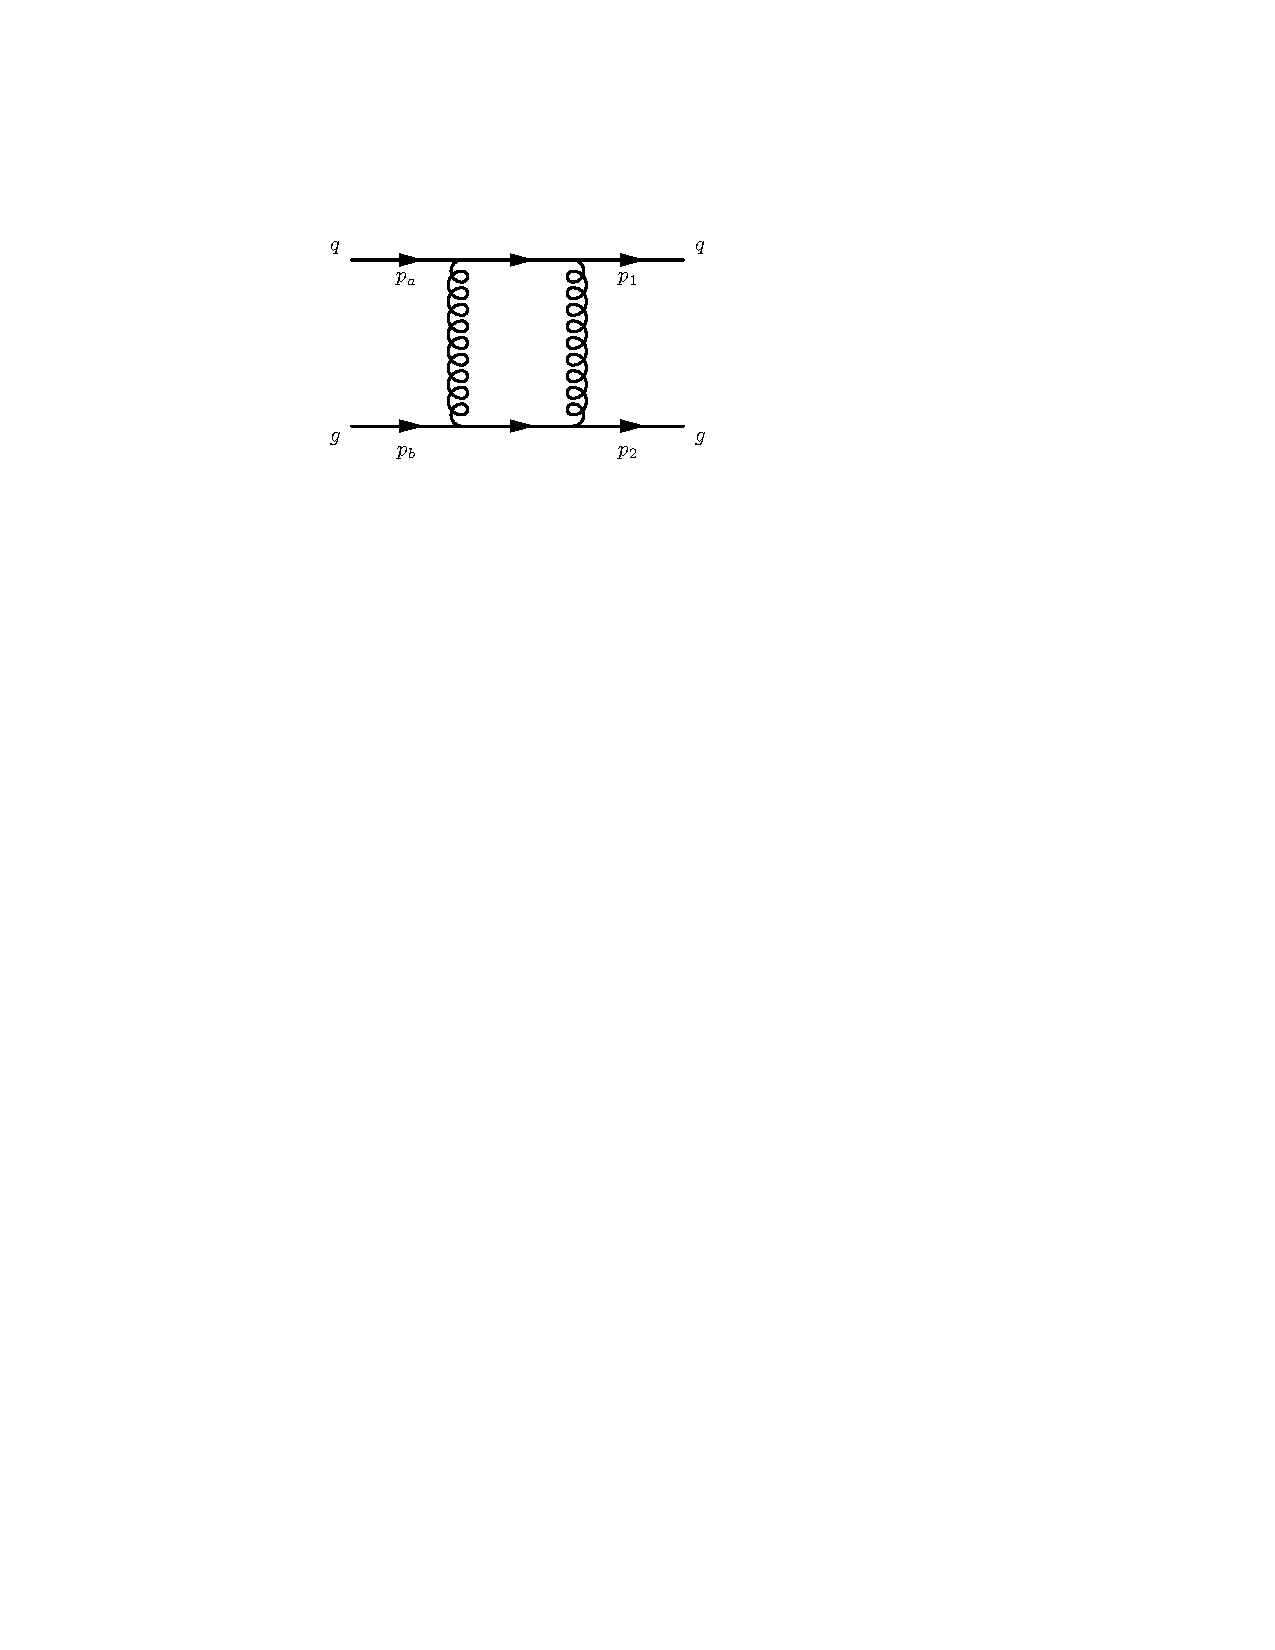
\includegraphics[width=0.8\textwidth]{NLO-uncrossed}
				\caption{}
				\label{fig:NLO-uncrossed}
			\end{subfigure}
			\begin{subfigure}[b]{0.48\textwidth}
				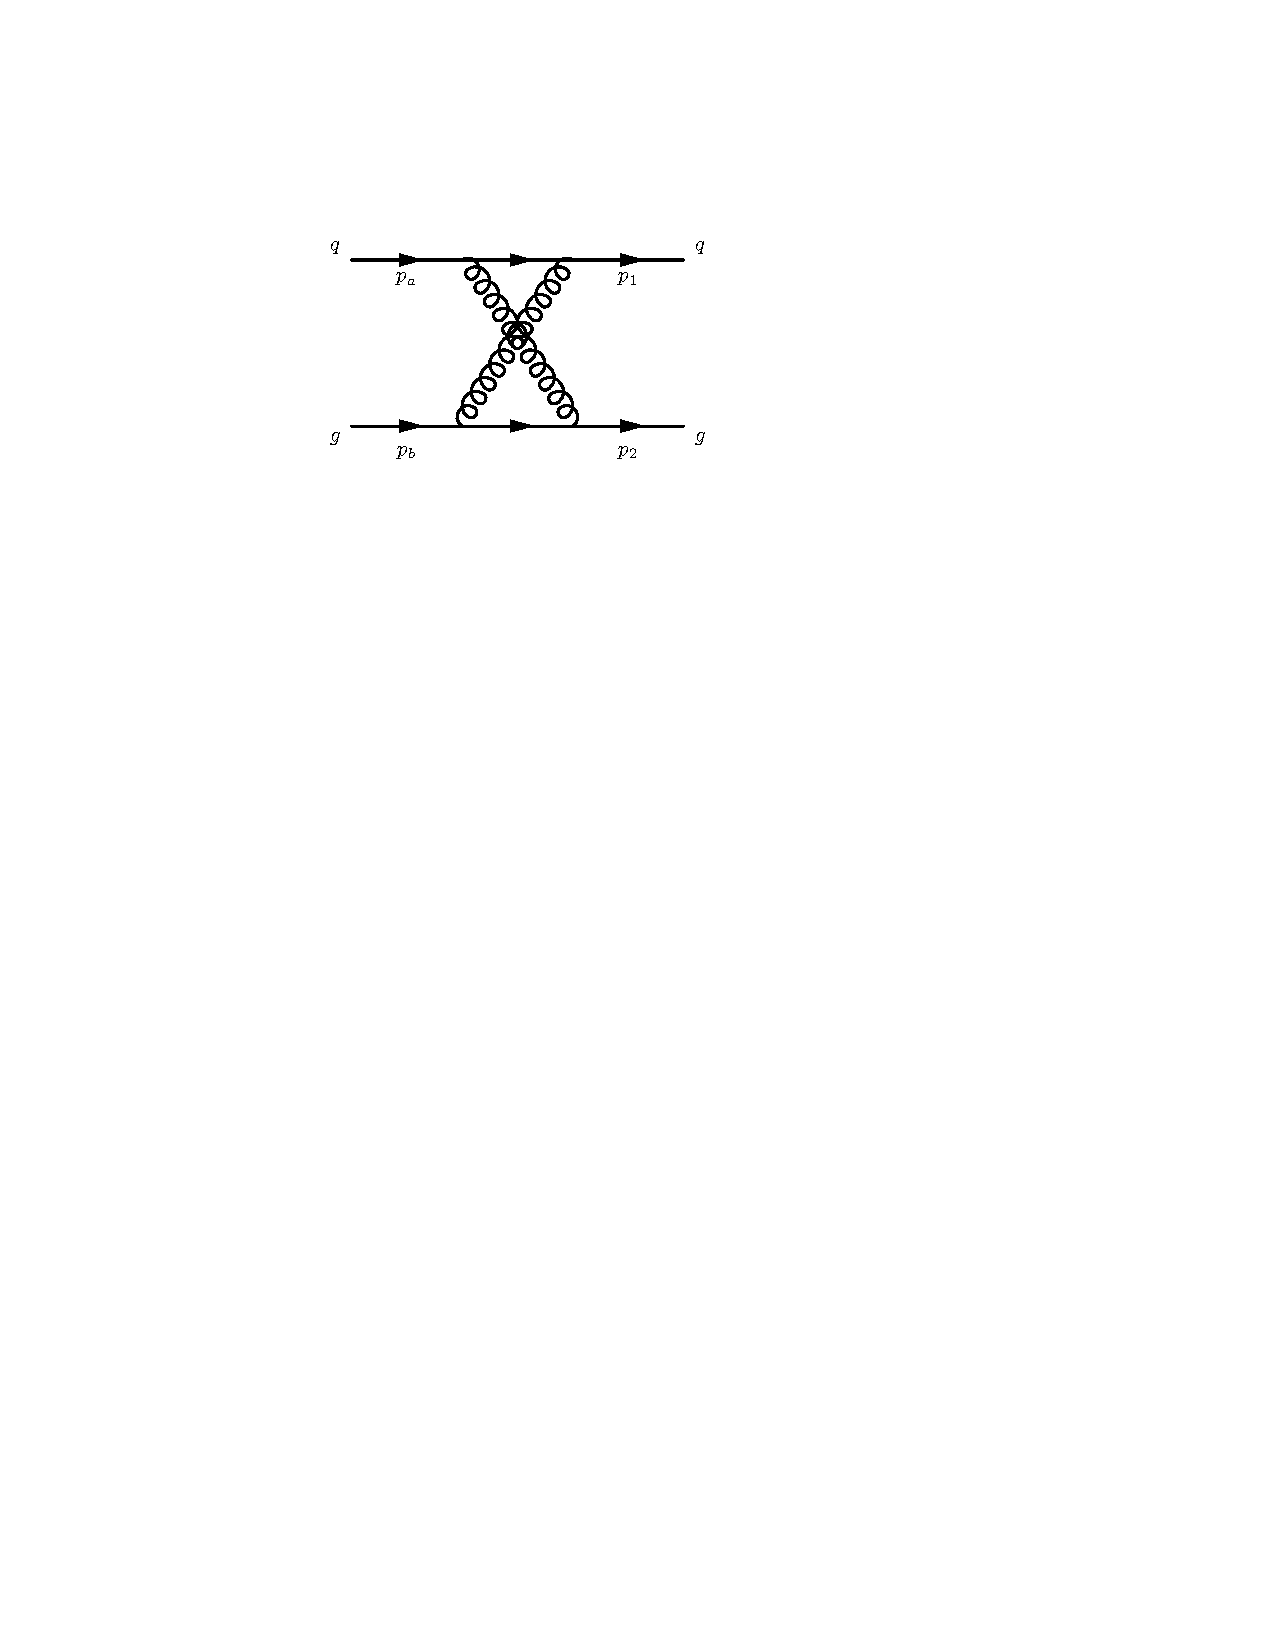
\includegraphics[width=0.8\textwidth]{NLO-crossed}
				\caption{}
				\label{fig:NLO-crossed}
			\end{subfigure}
			\caption{The leading logarithmic contributions to $qg\rightarrow qg$ at NLO.  The uncrossed
 			         diagram, $\mathcal{M}_{qQ\rightarrow qQ}^{\text{NLO}, II}$, shown in (a) exchanges
 			         two gluons in the $t$ channel and the crossed diagram,
 			         $\mathcal{M}_{qQ\rightarrow qQ}^{\text{NLO}, X}$, case (b) exchanges two gluons
 			         in the $u$ channel and is related to (a) (up to a colour factor) via a crossing
 			         symmetry}
			\label{fig:NLO-leadingContrib}
		\end{figure}

		\begin{equation}
			\mathcal{M}_{q^-Q^-\rightarrow q^-Q^-}^{\text{LO}} =
			-g_s^2T^d_{1a}T^d_{2b}\frac{\bk{1}{\mu}{a}\cdot\bk{2}{\mu}{b}}{t},
		\end{equation}

		as follows:

		\begin{align}
			\text{Im}\Big(\mathcal{M}_{qQ\rightarrow qQ}^{\text{NLO, II}}\Big) =
			\frac{1}{2(2\pi)^2}\int &d^4k\text{ }\delta((p_a-k)^2)
			\delta((p_b+k)^2)\\ &\mathcal{M}_{q^-Q^-\rightarrow q^-Q^-}^{\text{LO}}(k)
			\mathcal{M}_{q^-Q^-\rightarrow q^-Q^-}^{\dagger\text{LO}}(k-q),
		\end{align}

		where $\text{Im}(\cdot)$ denotes the imaginary part, $k$ is the loop momentum, $q$ is the momentum
		transfer and $\dagger$ denotes Hermitian conjugation.  In the High Energy limit we can perform the
		integration to give:

		\begin{equation}
			\text{Im}\Big(\mathcal{M}_{qQ\rightarrow qQ}^{\text{NLO, II}}\Big) =
			4\alpha_s^2 s\text{ }\mathcal{C}_1(T^a,T^b)
			\int \frac{dk_{\perp}}{k_{\perp}(k_{\perp} - q_{\perp})},
		\end{equation}

		where $\mathcal{C}_1(T^a,T^b)$ is the colour factor for the diagram and $k_{\perp}$ is the transverse
		component of $k$.  We can now relate the imaginary part of the amplitude to the full amplitude by
		conjecturing that the amplitude will be logarithmically enhanced as follows:

		\begin{align}
		\begin{split}
			\mathcal{M}_{qQ\rightarrow qQ}^{\text{NLO, II}} =
			&\text{Re}(\mathcal{M}_{qQ\rightarrow qQ}^{\text{NLO, II}}) +
			i\text{Im}(\mathcal{M}_{qQ\rightarrow qQ}^{\text{NLO, II}})\\
			:=&\widetilde{\mathcal{M}}_{qQ\rightarrow qQ}^{\text{NLO, II}}\ln\frac{s}{t} + \text{sub-leading}\\
			=&\widetilde{\mathcal{M}}_{qQ\rightarrow qQ}^{\text{NLO, II}}
			\ln\left|\frac{s}{t}\right| + \text{sub-leading},
			\label{eqn:rAndI}
		\end{split}
		\end{align}

		where we have used that $\frac{s}{t} < 0$.  Comparing real and imaginary parts of eqn.~\eqref{eqn:rAndI}
		and assuming that $\widetilde{\mathcal{M}}_{qQ\rightarrow qQ}^{\text{NLO, II}}$ is real we see that:

		\begin{equation}
			\text{Re}\Big(\mathcal{M}_{qQ\rightarrow qQ}^{\text{NLO, II}}\Big) =
			-\frac{1}{\pi}\text{Im}\Big(\mathcal{M}_{qQ\rightarrow qQ}^{\text{NLO, II}}\Big)
		\end{equation}

		and we can reconstruct the real part of the amplitude as:

		\begin{equation}
			\text{Re}\Big(\mathcal{M}_{qQ\rightarrow qQ}^{\text{NLO, II}}\Big) =
			-\frac{4\alpha_s^2u}{\pi} \mathcal{C}_1(T^a,T^b)
			\ln\left|\frac{u}{t}\right|\int \frac{dk_{\perp}}{k_{\perp}(k_{\perp} - q_{\perp})}.
			\label{eqn:uncrossedNLOcontrib}
		\end{equation}

		The crossed-diagram,~\eqref{fig:NLO-crossed}, also contributes a leading logarithmic piece and is related to
		eqn.~\eqref{fig:NLO-uncrossed} by a crossing symmetry and so we simply replace $u$ with $s$ in eqn.
		\eqref{eqn:uncrossedNLOcontrib} and calculate a new colour factor, $\mathcal{C}_2(T^a,T^b)$:

		\begin{equation}
			\text{Re}\Big(\mathcal{M}_{qQ\rightarrow qQ}^{\text{NLO, X}}\Big) =
			-\frac{4\alpha_s^2s}{\pi} \mathcal{C}_2(T^a,T^b)
			\ln\left|\frac{s}{t}\right| \int \frac{dk_{\perp}}{k_{\perp}(k_{\perp} - q_{\perp})}.
			\label{eqn:crossedNLOcontrib}
		\end{equation}

		But in the high energy limit $s\sim -u$ (this is clear from eqn.~\eqref{eqn:mandel2}) and so we
		can combine these terms and express the leading logarithmic NLO term in terms of the leading order
		result:

		\begin{equation}
			\mathcal{M}_{qQ\rightarrow qQ}^{\text{NLO}} = \frac{3\alpha_s}{\pi^2}
			\hat{\alpha}(q)\ln\left|\frac{s}{t}\right|
			\mathcal{M}_{qQ\rightarrow qQ}^{\text{LO}},
			\label{eqn:enhancedNLO}
		\end{equation}

		where:

		\begin{equation}
			\hat{\alpha}(q) = \int dk_{\perp}\frac{q_{\perp}^2}{k_{\perp}(k_{\perp} - q_{\perp})}
		\end{equation}

		From eqn.~\eqref{eqn:enhancedNLO} we can see the logarithmic enhancement explicitly; there is still
		a suppression from the inclusion of an extra factor of $\alpha_s$ with respect to the leading
		order term but as we have seen previously the logarithm is related to the kinematics of the final
		state - namely - the rapidity gap between the outgoing quarks $p_1$ and $p_2$ and compensate
		for the smallness of $\alpha_s$.

	\section{Effective Vertices For Real Emissions}
		\label{sec:effectiveVertices}

		In order to generalise what we have done so far to higher multiplicity scattering events we begin
		by considering $qQ\rightarrow qQg$ in the high energy limit.  The five diagrams which contribute at
		leading order are given in fig.~\eqref{fig:2To3}.  The diagram
		where the extra gluon is emitted from the $t$-channel gluon is given by:

		\begin{figure}[hbt]
			\begin{center}
			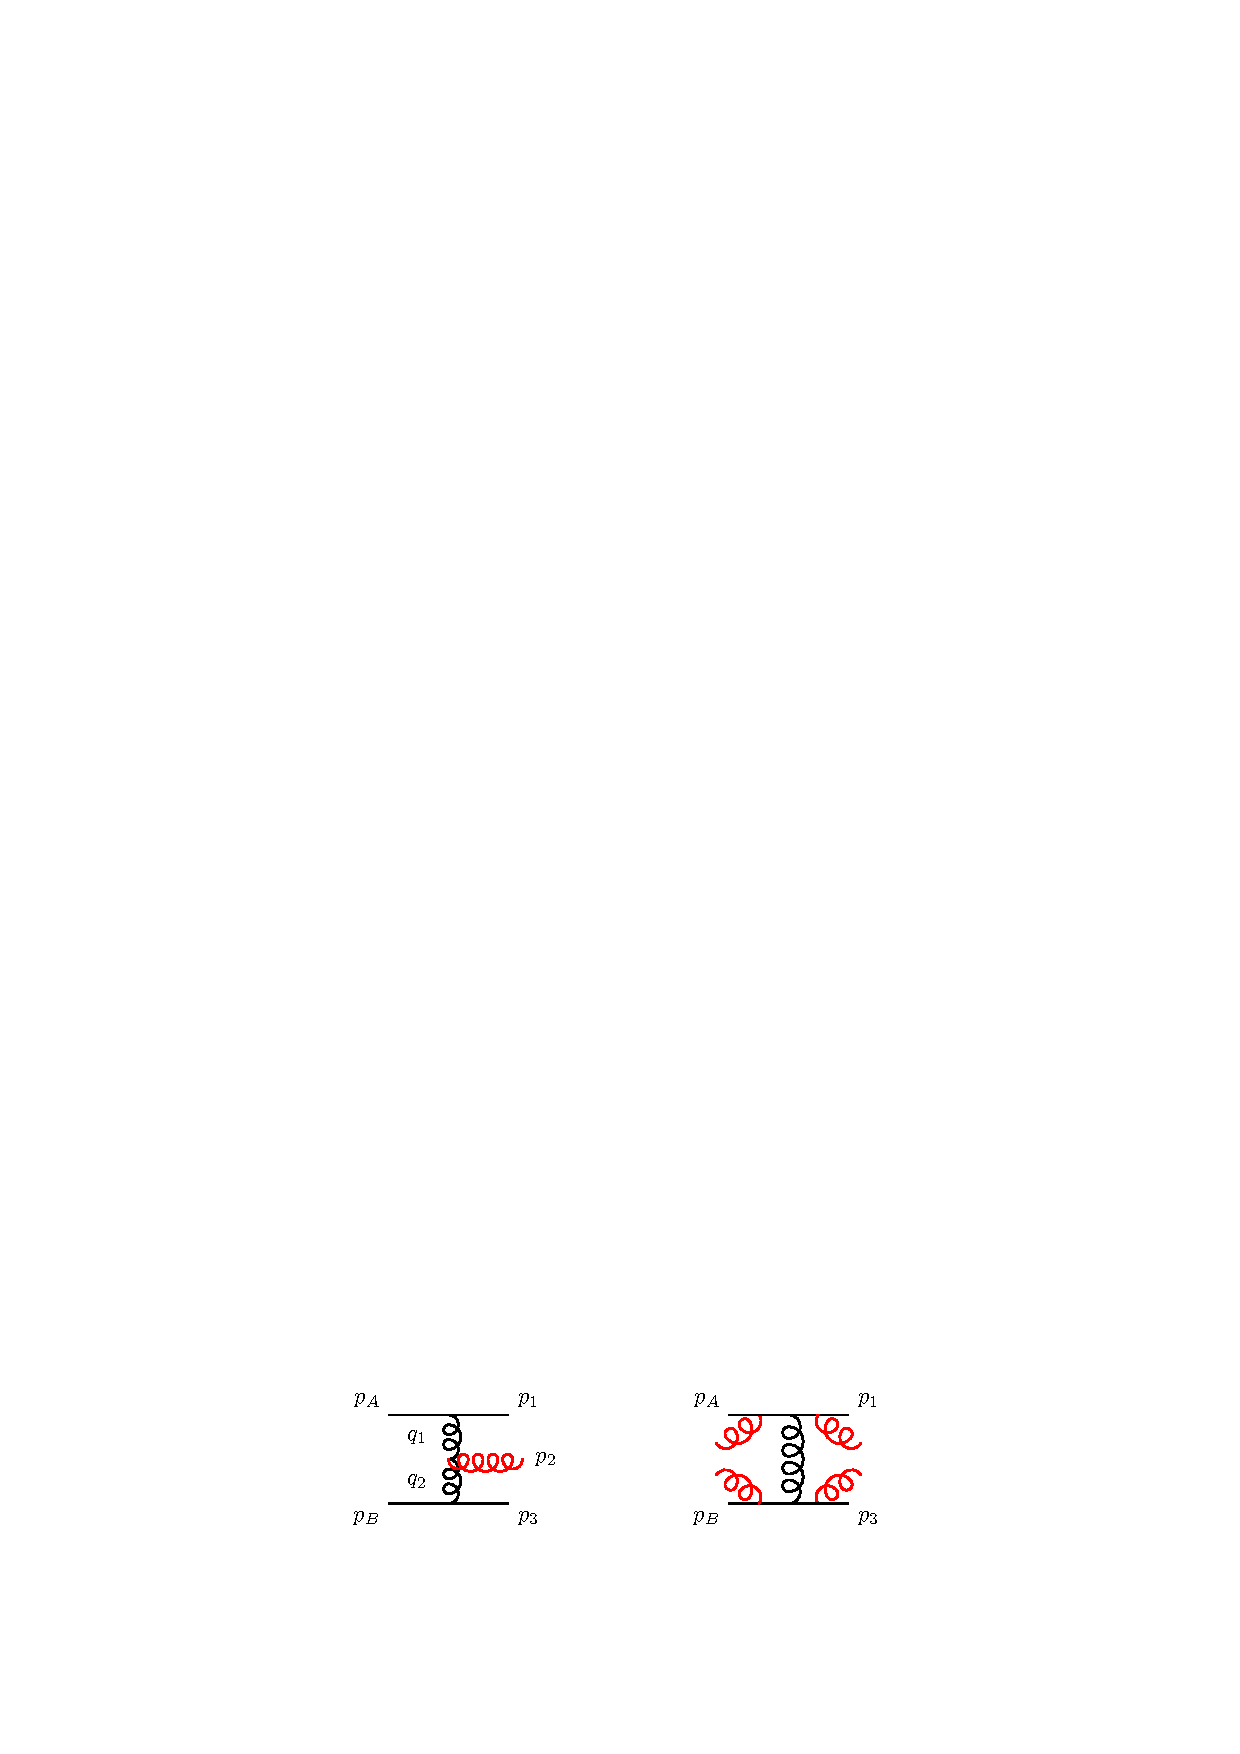
\includegraphics[width=0.7\linewidth]{2To3}
			\caption{The 5 possible emission sites of extra QCD radiation in $qQ\rightarrow qQ$.
			Fig. from \cite{Andersen:2009nu}.}
			\label{fig:2To3}
			\end{center}
		\end{figure}

		\begin{align}
		\begin{split}
			\mathcal{M}_{t\text{-channel}} = &-\frac{g_s^3}{t_{a1}t_{b2}}f^{i2j}T^i_{1a}T^j_{3b}\bk{1}{\rho}{a}\bk{3}{\mu}{b}
			\epsilon^*_{2\nu}\\&\left(2p_2^\mu g^{\nu\rho} - 2p_2^\rho g^{\mu\nu} - (q_1 + q_2)^\nu g^{\mu\rho} \right),
			\label{eqn:mtchannel}
		\end{split}
		\end{align}

		and the remaining four diagrams contribute like:

		\begin{align}
		\begin{split}
		    \mathcal{M}_{\text{Eik.}} = (ig_s)^3 \epsilon_{2\nu} \Bigg(
		     &T^2_{1i}T^d_{ia}T^d_{3b}\ \frac{2p_1^\nu\bk{1}{\mu}{a} + \bk{1}{\nu}{2}\bk{2}{\mu}{a}} {s_{12}t_{b3}} \bk{3}{\mu}{b} \\
		    +&T^d_{1i}T^2_{ia}T^d_{3b}\ \frac{2p_a^\nu\bk{1}{\mu}{a} - \bk{1}{\mu}{2}\bk{2}{\nu}{a}} {t_{a2}t_{b3}} \bk{3}{\mu}{b} \\
		    +&T^2_{3i}T^d_{ib}T^d_{1a}\ \frac{2p_3^\nu\bk{3}{\mu}{b} + \bk{3}{\nu}{2}\bk{2}{\mu}{b}} {s_{32}t_{a1}} \bk{1}{\mu}{a}\\
		    +&T^d_{3i}T^2_{ib}T^d_{1a}\ \frac{2p_b^\nu\bk{3}{\mu}{b} - \bk{3}{\mu}{2}\bk{2}{\nu}{b}} {t_{b2}t_{a1}} \bk{1}{\mu}{a}\Bigg).
			\label{eq:fulltree}
		\end{split}
		\end{align}

		In the High Energy limit the second term in each of the line is suppressed with respect to the
		first and can therefore be disregarded.  This turns out to be equivalent to if we considered
		$p_2$ as a soft emission using the Eikonal approximation.  The resulting amplitude for the sum
		of all four may be written in terms of the tree level amplitude as:

		\begin{align}
		\begin{split}
		    \mathcal{M}_{\text{Eik.}} = (ig_s)^3 \epsilon_{2\nu} \bk{1}{\mu}{a} \bk{3}{\mu}{b} \Bigg(
		     &T^2_{1i}T^d_{ia}T^d_{3b}\ \frac{2p_1^\nu}{s_{12}t_{b3}}
		    + T^d_{1i}T^2_{ia}T^d_{3b}\ \frac{2p_a^\nu}{t_{a2}t_{b3}} \\
		    +&T^2_{3i}T^d_{ib}T^d_{1a}\ \frac{2p_3^\nu}{s_{32}t_{a1}}
		    + T^d_{3i}T^2_{ib}T^d_{1a}\ \frac{2p_b^\nu}{t_{b2}t_{a1}}\Bigg).
			\label{eq:fulltree2}
		\end{split}
		\end{align}

		We now use that $p_a\sim p_1=p_+$ and $p_b\sim p_2=p_-$:

		\begin{align}
		\begin{split}
			\mathcal{M}_{\text{Eik.}} = (ig_s)^3 \epsilon_{2\nu} \bk{1}{\mu}{a} \bk{3}{\mu}{b} \Bigg(&
			\frac{2p_+^\nu}{p_+\cdot p_2 t_{b3}}(T^2_{1i}T^d_{ia} - T^d_{1i}T^2_{ia})T^d_{3b}\\
			+ &\frac{2p_-^\nu}{p_-\cdot p_2 t_{a1}}(T^2_{3i}T^d_{ib} - T^d_{3i}T^2_{ib})T^d_{1a}\Bigg).\\
		\end{split}
		\end{align}

		Now tidying up the colour factors:

		\begin{align}
		\begin{split}
			\mathcal{M}_{\text{Eik.}} = (ig_s)^3 \epsilon_{2\nu} \bk{1}{\mu}{a} \bk{3}{\mu}{b}
			f^{2de}T^b_{3b}T^e_{1a}\frac{1}{t_{a1}t_{b3}}\Bigg(&
			\frac{2p_+^\nu}{p_+\cdot p_2}t_{a1} - \frac{2p_-^\nu}{p_-\cdot p_2}t_{b3}\Bigg),
			\label{eq:fulltree3}
		\end{split}
		\end{align}

		which has a colour factor similar to that found for the diagrams with a gluon emitted from the
		$t$-channel gluon.  We choose to `symmetrise' eqn.~\eqref{eqn:fulltree3} by returning to $p_{a/1}$
		and $p_{b/3}$ explicitly in place of $p_+$ and $p_-$ respectively:

		\begin{align}
		\begin{split}
			\mathcal{M}_{\text{Eik.}} = &(ig_s)^3 \epsilon_{2\nu} \bk{1}{\mu}{a} \bk{3}{\mu}{b} f^{2de}T^b_{3b}T^e_{1a}\frac{1}{t_{a1}t_{b3}}\\
			&\half\Bigg(\frac{2p_a^\nu}{p_a\cdot p_2}t_{a1} + \frac{2p_1^\nu}{p_1\cdot p_2}t_{a1} -
			\frac{2p_b^\nu}{p_b\cdot p_2}t_{b3} - \frac{2p_3^\nu}{p_3\cdot p_2}t_{b3}\Bigg).
			\label{eq:fulltree4}
		\end{split}
		\end{align}

		We now consider~\eqref{eqn:mtchannel}.  The final term contracts the two currents and so it is
		only the first two terms which need to be massaged into the right form.  Once again we
		approximate using $p_a\sim p_1=p_+$ and $p_b\sim p_3=p_-$ to write the currents as momenta.
		Upon doing this we find:

		\begin{align}
		\begin{split}
			\mathcal{M}_{t\text{-channel}} = &-\frac{g_s^3}{t_{a1}t_{b2}}f^{i2j}T^i_{1a}T^j_{3b} \epsilon^*_{2\nu} \\
			&\left(8e^{i\phi_-}(p_+^\nu p_-\cdot p_2 - p_-^\nu p_+\cdot p_2) - (q_1 + q_2)^\nu \bk{1}{\mu}{a}\bk{3}{\mu}{b} \right),
			\label{eqn:mtchannel2}
		\end{split}
		\end{align}

		where $\phi_-$ is a phase resulting from the spinor conventions detailed in chapter~\ref{chap:theory}.
		Now using that $s\sim2p_+\cdot p_-=\half\bk{1}{\mu}{a}\bk{3}{\mu}{b}e^{-i\phi_-}$ we can write all
		three terms as something proportional to the desired current structure:

		\begin{align}
		\begin{split}
			\mathcal{M}_{t\text{-channel}} = &-\frac{g_s^3}{t_{a1}t_{b2}}f^{i2j}T^i_{1a}T^j_{3b} \epsilon^*_{2\nu}
			\bk{1}{\mu}{a}\bk{3}{\mu}{b} \\&\left(4\left(p_+^\nu \frac{p_-\cdot p_2}{s} - p_-^\nu \frac{p_+\cdot p_2}{s}\right)
			- (q_1 + q_2)^\nu \right).
			\label{eqn:mtchannel3}
		\end{split}
		\end{align}

		Similarly as for $\mathcal{M}_{\text{Eik.}}$ we chose to include as much of the actual
		kinematic information as possible by symmetrising~\eqref{eqn:mtchannel3} to get:

		\begin{align}
		\begin{split}
			\mathcal{M}_{t\text{-channel}} = &-\frac{g_s^3}{t_{a1}t_{b2}}f^{i2j}T^i_{1a}T^j_{3b} \epsilon^*_{2\nu}
			\bk{1}{\mu}{a}\bk{3}{\mu}{b}\\
			&\Bigg(-(q_1 + q_2)^\nu + \half\Big(
			p_a^\nu \frac{p_2\cdot p_b}{p_a\cdot p_b} + p_a^\nu \frac{p_2\cdot p_3}{p_a\cdot p_3} +
			p_1^\nu \frac{p_2\cdot p_b}{p_1\cdot p_b} + p_1^\nu \frac{p_2\cdot p_3}{p_1\cdot p_3}  \\
		       &-p_b^\nu \frac{p_2\cdot p_a}{p_a\cdot p_b} - p_b^\nu \frac{p_1\cdot p_2}{p_b\cdot p_1} -
			p_2^\nu \frac{p_2\cdot p_a}{p_a\cdot p_3} - p_2^\nu \frac{p_1\cdot p_2}{p_1\cdot p_3}
			\Big)
			\Bigg).
			\label{eqn:mtchannel4}
		\end{split}
		\end{align}

		Since eqns.~\eqref{eqn:mtchannel4} and~\eqref{eq:fulltree4} to the same colour factor we can simply sum
		them to get:

		\begin{equation}
			\mathcal{M}_{qQ\rightarrow qQg} = \frac{S_{qQ\rightarrow qQ}}{t_{a1}t_{b2}}
			f^{2de}T^b_{3b}T^e_{1a}g_s^3\epsilon^*_\rho V_\rho(q_1, q_2),
		\end{equation}

		where

		\begin{align}
			V^\rho(q_1, q_2) = -(q_1 + q_2)^\rho +
			&\frac{p_a^\rho}{2}\left(\frac{q^2_1}{p_a\cdot p_2} + \frac{p_2 \cdot p_b}{p_a \cdot p_b} +
			\frac{p_2 \cdot p_3}{p_a \cdot p_3}\right) + (p_a\leftrightarrow p_1) \\
			- &\frac{p_b^\rho}{2}\left(\frac{q^2_2}{p_b\cdot p_2} + \frac{p_2 \cdot p_a}{p_a \cdot p_b} +
			\frac{p_2 \cdot p_1}{p_b \cdot p_1}\right) - (p_b\leftrightarrow p_3).
			\label{eqn:effVertex}
		\end{align}

		Eqn.~\eqref{eqn:effVertex} is manifestly gauge invariant which can be checked explicitly by
		calculating $p_g\cdot V$.  It is, however clearly divergent:  if any of $p_a$, $p_b$, $p_1$,
		$p_2$ or $p_3$ becomes soft then the momenta contractions in the denominators of eqn.
		\eqref{eqn:effVertex} will become zero and the whole expression will explode.  We organise
		the cancellation of divergences is shown to cancel in the following chapter.

		Armed with eqn.~\eqref{eqn:effVertex} and the quark and gluon currents we can calculate
		high multiplicity matrix elements by generalising eqn.~\eqref{eqn:factorised} to include
		contractions of this effective vertex expression.  The $2\rightarrow n$ matrix element
		squared for $qQ$ scattering is therefore given by:

		\begin{align}
		\begin{split}
			|\overline{\mathcal{M}}^t_{qQ\rightarrow qg\cdots gQ}|^2 = \frac{1}{4(N_c^2-1)}
			\frac{g^2C_F}{t_1}\frac{g^2C_F}{t_2} \sum_{h_a, h_b, h_1, h_2}
			|S_{qQ\rightarrow qQ}^{h_ah_b\rightarrow h_1h_2}|^2\\
			\times\prod_{i=1}^{n-1}\left(\frac{-g_sC_A}{t_it_{i+1}}V^\mu(q_i, q_{i+1})V_\mu(q_i, q_{i+1})\right).
			\label{eqn:factorised2ToN}
		\end{split}
		\end{align}

		Using eqn.~\eqref{eqn:factorised2ToN} we can describe the real emission high order
		corrections but this expression is manifestly divergent for the reasons outlined in
		section \ref{sec:divAndReg}.  As in section~\ref{sub:eg1loop} we must calculate the
		virtual corrections to render the integrated cross section finite.

	\section{Virtual Corrections To All Orders}
		\label{sub:virtuals}

		In the High Energy limit we may include the virtual corrections to all orders in $\alpha_s$ by using
		the Lipatov ansatz \cite{Kuraev:1976ge}.  For $t$-channel gluons we replace the usual
		gluon propagator:

		\begin{equation}
			\frac{1}{q_i^2},
		\end{equation}

		with a `dressed' version given by:

		\begin{equation}
			\frac{1}{q_i^2}e^{\hat{\alpha}(q_i)\Delta_{i,i-1}},
		\end{equation}

		where:

		\begin{equation}
			\hat{\alpha}(q_i) = \alpha_sC_Aq_i^2\int \frac{d^{2+2\epsilon}k_{\perp}}{(2\pi)^{2+2\epsilon}}
			\frac{1}{k^2_\perp(k_\perp - q_{i\perp})^2}\mu^{-2\epsilon},
		\end{equation}

		and $\Delta_{i,i-1}$ is the rapidity gap between the external gluon legs emitted from
		the dressed gluon.  Similarly to eqn.~\eqref{eqn:effVertex} in the preceding section this
		new expression for the propagator contains divergences arising from the soft limit
		of the integral in the expression for $\hat{\alpha}(q_i)$.  In the following chapter we
		show in some detail that these divergences cancel with those mentioned in section
		\ref{sec:effectiveVertices}.

\chapter{High Energy Jets}
\label{chap:HEJ}

	{\color{red}
	\begin{itemize}
		\item HEJ codebase
		\item Current predictions
		\item What else can go here...
		\item Combined code discussion?
		\item J/W/H comparisons to data?
	\end{itemize}
	}

	\section{The \HEJ Framework}

	\section{Comparisons to Data}

	\section{Matching to \ARIADNE}

